\documentclass[10pt , a4paper]{report}
% The preceding line is only needed to identify funding in the first footnote. If that is unneeded, please comment it out.
% \usepackage[T2A,T1]{fontenc}
\usepackage{silence}

\usepackage{cite}
\usepackage{amsmath,amssymb,amsfonts}
\usepackage{algorithmic}
\usepackage{graphicx}
\usepackage{listings}
\usepackage{textcomp}
\usepackage{sectsty}
\usepackage{xcolor}
\usepackage{appendix}
\def\BibTeX{{\rm B\kern-.05em{\sc i\kern-.025em b}\kern-.08em
    T\kern-.1667em\lower.7ex\hbox{E}\kern-.125emX}}

\usepackage[utf8x]{inputenc}
\usepackage[english,russian]{babel}
\usepackage{cmap}

\usepackage{titlesec}
\titleformat{\chapter}
  {\normalfont\LARGE\bfseries}{\thechapter}{1em}{}
\titlespacing*{\chapter}{0pt}{3.5ex plus 1ex minus .2ex}{2.3ex plus .2ex}

%paragraphs params
\setlength{\oddsidemargin}{0cm}
\setlength{\textheight}{24cm}
\setlength{\textwidth}{16cm}
\setlength{\topmargin}{-2cm}
\renewcommand{\baselinestretch}{1.1}

% fonts
\usepackage{times}
\usepackage{helvet} 
\usepackage{sectsty}
\allsectionsfont{\sffamily}
\renewcommand{\familydefault}{\sfdefault}


%listings
\lstset{basicstyle=\ttfamily\footnotesize}
\lstset{frame=tlrb}
\usepackage{listings}

\usepackage{minted}

\usepackage{adjustbox}
\usepackage{subcaption}
\captionsetup{compatibility=false}


\begin{document}

\title{Computer Science Project\\
        \textit{Kandy: CLI tool for managing Kafka}}

\author{\textbf{Alex Lukin}\\
Chesterton Community College\\
\textit{Cambridge, United Kingdom}\\}


\maketitle

\newpage
\tableofcontents
\newpage

\chapter{Analysis}
\section{Problem Definition}

Apache Kafka\footnote{\textbf{Kafka} is a distributed streaming platform designed for processing, storing, and transmitting data in real-time. It provides a reliable mechanism for data streaming, enabling applications and services to exchange information and respond to changes instantly. Kafka is built to handle enormous volumes of data, offering high performance and fault tolerance through its distributed architecture.} has become a crucial system for handling real-time data streams in today’s data-driven landscape. Despite Kafka’s widespread adoption, there remains a lack of streamlined tools for efficient management of Kafka instances directly from the command line. This gap poses a challenge for developers who need quick, straightforward ways to interact with Kafka without getting slowed down by complex setup processes.

While web applications can bridge this gap by providing intuitive interfaces, they are typically hosted in Docker containers. Docker’s benefits of portability and consistency across different environments are valuable, yet setting up these applications within large systems can become cumbersome and time-consuming, especially for quick local tests.

In summary, Docker facilitates deploying web applications with user-friendly interfaces for Kafka management, but its setup can be daunting within larger infrastructures. To address this, the proposed solution is a dedicated Text-Based User Interface (TUI) utility aimed at simplifying Kafka management, ultimately boosting developer productivity.

The project is named \textbf{Kandy}(Stands for Handy Kafka) and is envisioned as a TUI tool specifically designed for Kafka management

\section{Stakeholders} 
The Kandy project targets three primary stakeholder groups, each with distinct needs that Kandy will address:

\begin{itemize} 
    \item \textbf{Administrators} who oversee Kafka performance, data integrity, and cluster health. Kandy’s real-time monitoring features provide quick insights into cluster status, helping administrators maintain stability and react swiftly to any issues.
    \item \textbf{Developers} who integrate Kafka into their applications and require efficient access to Kafka for testing, debugging, and troubleshooting. Kandy streamlines access to critical metrics, enhancing their productivity and reducing setup time for Kafka-related tasks.
    \item \textbf{DevOps teams} responsible for Kafka cluster infrastructure, uptime, and stability. Kandy’s intuitive interface and essential monitoring tools enable DevOps teams to oversee cluster health without the need for complex GUI-based solutions, making management tasks more efficient.
\end{itemize}

To represent the target audience, I have identified a key user persona: \textbf{Sarah}, the Head of Engineering at Valerann. Sarah oversees multiple data-driven projects that rely on real-time Kafka streams, frequently monitoring consumer lags, topic performance, and system stability to ensure smooth operation for her teams. With extensive experience in both development and Kafka management, Sarah’s insights are invaluable for evaluating Kandy’s effectiveness. Sarah’s feedback will help me to be sure if Kandy meets the practical needs of it's users.

\newpage

\section{Kafka Architecture}

Throughout whole project, I will use terminology specific to Kafka’s architecture to describe its components and functionalities. So
this subsection dives into the foundational concepts of Kafka. For better understanding the key ideas behind Kafka and its functionality, let’s break it down into its core components and how they work together.

\begin{figure}[htbp]
    \centering
    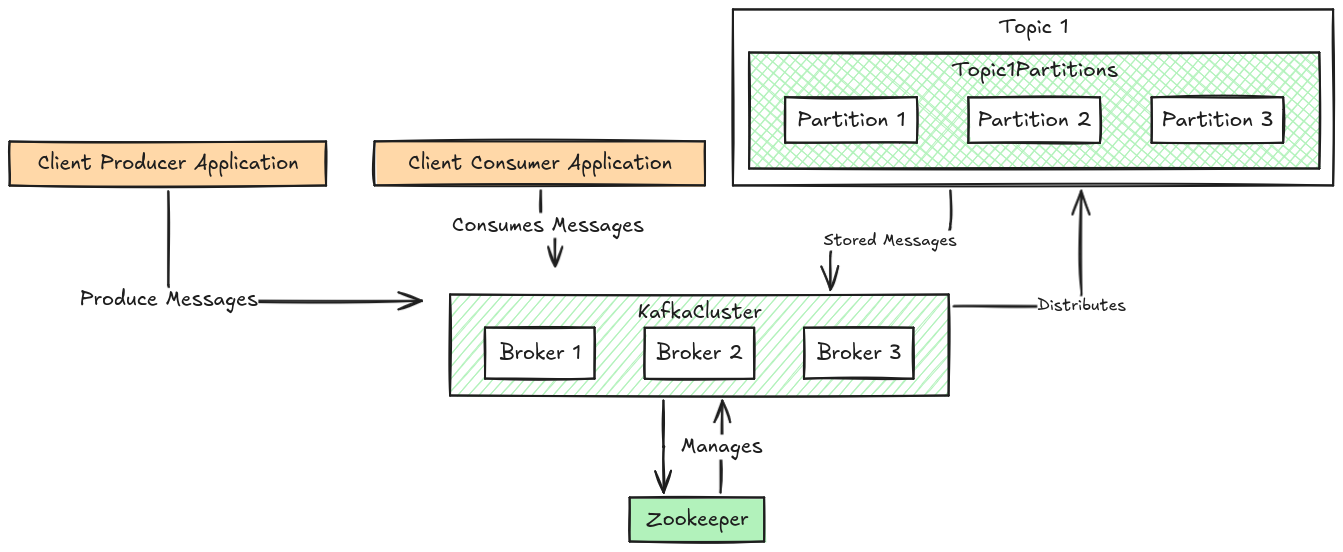
\includegraphics[width=1\linewidth]{imgs/KafkaStructureModel.png}
    \caption{Key Components of Kafka Architecture}
    \label{fig:kafka_arch}
\end{figure}

\subsubsection*{Core Components of Kafka}
\begin{itemize}
    \item \textbf{Message:} The fundamental unit of data in Kafka. It consists of a key, value, and optional metadata (headers)
    
    \textit{Example:} A message in the \textit{Weather\_Updates} topic might include a key representing a city ID, a value containing temperature data, and headers indicating the time of measurement.
    
    \item \textbf{Producers:}  
    These are the data generators. Producers are applications or systems responsible for sending messages to Kafka topics. Think of them as the "writers" in Kafka's ecosystem. 
    
    \textit{Example:} A weather monitoring application sending real-time temperature updates acts as a producer.

    \item \textbf{Consumers:}  
    Consumers retrieve and process data stored in Kafka topics. They are the "readers" that transform raw data into actionable insights or visualizations.  
    
    \textit{Example:} A live dashboard showing weather updates would be a consumer.

    \item \textbf{Topics and Partitions:}  
    \begin{itemize}
        \item \textbf{Topics:} Logical containers that organize messages by category. For instance, a topic named \textit{Weather\_Updates} might store all weather-related data.
        \item \textbf{Partitions:} Subsections of a topic that allow for parallel processing. Each partition stores messages in an immutable, sequential order. This setup enables Kafka to scale efficiently by distributing messages across multiple servers (brokers).
    \end{itemize}

    \item \textbf{Brokers:}  
    Brokers are Kafka's backbone. They store data and manage partitions. When combined, multiple brokers form a Kafka cluster, which offers high availability and fault tolerance by replicating and balancing data across servers.

    \item \textbf{Zookeeper:}  
    Zookeeper is a distributed coordination service crucial to Kafka's operations. It tracks metadata, manages partition leadership, and monitors broker health to ensure cluster stability. Although Zookeeper is essential in Kafka’s traditional setup, newer Kafka versions are moving towards its replacement with Kafka's internal \textit{KRaft} system.  
    \textit{(Note: I'm not planning on working with Zookeeper directly in this project, but understanding its role might be helpful)}
\end{itemize}

\subsubsection*{How Kafka Works}
\begin{enumerate}
    \item \textbf{Producers Generate Data:}  
    Applications acting as producers send data to Kafka, specifying the relevant topic. For instance, a weather app might publish updates to a \textit{Weather\_Updates} topic.

    \item \textbf{Kafka Distributes Data Across Partitions:}  
    Kafka divides incoming data into partitions within a topic and distributes these partitions across brokers in the cluster. This design allows efficient load balancing and supports simultaneous access by multiple consumers.

    \item \textbf{Consumers Process Data:}  
    Consumers subscribe to topics and retrieve data from specific partitions. Kafka ensures that data can be processed in parallel, enabling high-performance real-time analytics or other operations.
\end{enumerate}

\section{Computational Methods}

Managing Apache Kafka, a distributed and data-intensive system, requires careful application of computational methods. Kafka's complex architecture involves intricate interactions between brokers, topics, partitions, and consumers. Computational approaches simplify this complexity, making it feasible to develop a Text-Based User Interface (TUI) that provides users with an intuitive way to manage Kafka. This section outlines how principles such as \textit{Abstraction}, \textit{Decomposition}, \textit{Thinking Ahead}, and \textit{Algorithmic Thinking} are employed in the development of the TUI.

\subsection{Abstraction}

\subsubsection*{Definition:}  
Abstraction simplifies a complex system by emphasizing its essential features while hiding less relevant details.

\subsubsection*{Application:}  
Abstraction is at the heart of this TUI’s design, allowing users to interact with Kafka’s core components—brokers, topics, partitions, and consumer groups—without requiring deep knowledge of Kafka’s APIs or internal mechanisms. The TUI abstracts Kafka’s functionalities into high-level commands and representations:
\begin{itemize}
    \item \textbf{Brokers:} Represented as nodes with health status and connectivity information.
    \item \textbf{Topics:} Abstracted as logical containers for message streams, with partition and replication details available upon request.
    \item \textbf{Consumers:} Displayed as groups subscribing to topics, with key metrics such as consumer lag simplified for clarity.
\end{itemize}

This abstraction ensures that even novice users can perform critical Kafka operations, such as topic creation, monitoring, and deletion, using an accessible interface.

\subsection{Decomposition}

\subsubsection*{Definition:}  
Decomposition breaks a large, complex problem into smaller, manageable sub-problems.

\subsubsection*{Application:}  
The development of the TUI leverages decomposition to divide Kafka management into specific functional components:
\begin{itemize}
    \item \textbf{Topic Management:} Includes operations such as creating, deleting, and listing topics with detailed configurations.
    \item \textbf{Consumer Monitoring:} Tracks consumer groups, displays subscription details, and monitors consumer lag.
    \item \textbf{Broker Status Monitoring:} Reports on broker health and displays connectivity details.
\end{itemize}

Each component is further divided into smaller tasks. For example, ``Topic Management'' includes sub-tasks like validating topic names, setting replication factors, and handling partition assignments. Decomposition makes the project more manageable, enables iterative development, and allows for parallelization of work across different modules.

\subsection{Thinking Ahead}

\subsubsection*{Definition:}  
Thinking Ahead involves anticipating future needs and ensuring the solution is robust and scalable.

\subsubsection*{Application:}  
The TUI is designed with extensibility in mind, anticipating potential changes in Kafka’s architecture and user requirements. For instance:
\begin{itemize}
    \item The TUI supports dynamic configuration, allowing it to adapt to changes in the number of brokers or topics without significant modifications.
    \item Modular code design ensures that new features, such as support for Kafka Streams or advanced monitoring tools, can be integrated seamlessly.
\end{itemize}

By thinking ahead, the TUI ensures long-term usability and minimizes maintenance efforts, even as Kafka evolves.

\subsection{Algorithmic Thinking}

\subsubsection*{Definition:}  
Algorithmic Thinking involves designing and implementing efficient, logical steps to solve a problem.

\subsubsection*{Application:}  
Several features of the TUI rely on algorithmic thinking:
\begin{itemize}
    \item Efficient algorithms for calculating consumer lag ensure that real-time metrics are displayed without significant delays.
    \item Partition assignment algorithms optimize how messages are distributed across brokers, ensuring load balancing.
    \item Sorting and filtering operations in the TUI enable users to quickly locate relevant topics or consumers, even in large Kafka clusters.
\end{itemize}

These algorithmic enhancements ensure that the TUI provides accurate and responsive feedback, critical for managing a live distributed system.

\subsection{Evaluation and Refinement}

As part of the computational process, evaluation and refinement ensure that the TUI meets user needs effectively. Continuous testing is performed to verify:
\begin{itemize}
    \item Usability: Ensuring the interface remains intuitive for users with varying levels of experience.
    \item Performance: Verifying that the TUI scales efficiently with large Kafka clusters.
    \item Correctness: Ensuring that operations, such as topic creation or consumer monitoring, produce accurate results.
\end{itemize}

\subsection{Conclusion}

By applying computational methods such as abstraction, decomposition, thinking ahead, and algorithmic thinking, the TUI simplifies Kafka management for users. These principles ensure that the solution is user-friendly, scalable, and adaptable to future requirements, demonstrating the importance of computational methods in solving complex, real-world problems.


\chapter{Research}
\section{Interview questions}

I will outline here key questions that I will ask stakeholder, but during the interview I may come up with follow up questions. The interview will help me find their opinion on the software and how they would like to use it.

\subsection{Questions}
\begin{itemize}
    \item \textbf{How often do you work with Kafka? What utilities do you use to work with it? Why those?}
        \begin{itemize}
            \item Understanding the frequency of interaction with Kafka is crucial for designing a utility that meets the stakeholder's needs without overwhelming them with unnecessary features
        \end{itemize}
    \item \textbf{Can you describe in detail the last problem you solved related to Kafka?}
    \begin{itemize}
            \item Gathering detailed information about recent challenges helps in designing features and functionalities within the utility to address common pain points
    \end{itemize}
    \item \textbf{Is there anything you're currently dissatisfied with in the utilities you use? What would you change?}
        \begin{itemize}
            \item Discovering dissatisfaction with existing utilities guides the development of the utility by focusing on areas for improvement or enhancement
            \item Knowing desired changes informs feature prioritisation, ensuring that the utility aligns with stakeholder expectations and addresses their specific pain points effectively
        \end{itemize}
    \item \textbf{Do you have a preference for a Terminal User Interface (TUI) or web-based solution for managing Kafka? If so, what are the reasons behind your preference?}
        \begin{itemize}
            \item Understanding stakeholders' preferences for either a Terminal User Interface or web-based solution provides crucial insights into their workflow preferences and the environment in which they operate. This information ensures that the utility is developed in a manner that seamlessly integrates into their existing workflows, ultimately enhancing user experience and satisfaction
        \end{itemize}
    \item \textbf{Describe the recent problems you encountered while using <Name of the utilities>}
        \begin{itemize}
            \item Identifying areas of dissatisfaction with current utilities allows for targeted improvements in the design and functionality of the TUI utility. By addressing these pain points, the TUI utility can be tailored to better meet the needs and expectations of stakeholders, resulting in a more effective and user-friendly solution.
        \end{itemize}
        
    \item \textbf{What do you believe would be the ideal number of clusters the system should handle simultaneously? Why? How many clusters have you worked with simultaneously in the past?}
        \begin{itemize}
            \item Understanding the optimal number of clusters for concurrent support is key to ensuring the system scales seamlessly and manages resources efficiently.
        \end{itemize}
    \item \textbf{Could you explain how you currently configure connections to the clusters, and how user-friendly do you find this process?}
        \begin{itemize}
            \item Understanding how connections to the clusters are currently configured and evaluating the user-friendliness of this process can provide valuable insights, ensuring that the new utility addresses any shortcomings and provides a seamless user experience.
        \end{itemize}
    \item \textbf{When thinking about how data from the clusters is displayed, what are your main expectations? For example, how quickly data is presented by current tools, and how satisfied are you with this?}
        \begin{itemize}
            \item Understanding the expectations regarding data display from the clusters is crucial for informing development priorities and ensuring alignment with stakeholder needs and by gaining insights into these aspects, we can effectively prioritise features and enhancements within the utility
        \end{itemize}
    \item \textbf{Can you describe some common scenarios where you would use multiple clusters? For instance, comparing data across different topics or any other important scenarios you have in mind?}
        \begin{itemize}
            \item Understanding common scenarios where users would use multiple clusters is important for designing a utility that meets users’ needs effectively. By considering these scenarios, I can ensure that the utility is versatile enough to support a wide range of users workflow needs
        \end{itemize}
\end{itemize}


\section{Interview}


\subsection*{Can you please introduce yourself and describe your experience with Kafka?}

Sure. My name is Sarah Anderson, and I’m the Head of Engineering at Valerann. I’ve been with the company for nearly three years, and I’ve been working in tech for almost ten years. Regarding my experience with Kafka, I started using it about six years ago while working at a marketing technology company. They used Kafka to process large volumes of email notifications and automatically convert them into sales. Since then, I’ve worked with Kafka in about five different companies, all primarily for high-volume, real-time data processing.

Typically, my role with Kafka has involved helping companies implement and scale it from the ground up. Kafka provides excellent scalability, but transitioning from a traditional monolithic architecture to an event-driven, Kafka-based design requires significant effort. Developers often need training, and management needs to understand how to structure and scale a Kafka architecture. I’ve spent much of my time helping teams learn how to use Kafka, build systems around it, and implement it effectively.

\subsection*{How often do you work with Kafka now, and what utilities and tools do you use to manage it?}

Currently, I work with Kafka every few days—around three times a week. However, I don’t interact with the individual services as much as I used to. In terms of tools, we primarily use a tool called Faust Streaming, which was derived from an older tool called Faust (created by a company called Robinhood, not to be confused with the Bitcoin company). However, Faust is now deprecated, and we’re moving away from it. We’ve been using it as our streaming framework, similar to the Kafka Streams Java framework but written in Python—and not as efficiently. We're gradually replacing it with an in-house tool we’ve developed called CitizenK (inspired by the movie \textit{Citizen Kane} and Kafka's initial).

For managing Kafka day-to-day, we use an open-source tool from Provectus Labs that provides a free UI for administering Kafka clusters, performing tasks like cleaning up consumer groups or resetting offsets. For infrastructure management, we use Terraform to create clusters, brokers, topics, and set up initial settings.

\subsection*{Can you describe any problems you've encountered while using these tools to manage Kafka?}

One of the most common issues we face with admin tools is the lack of effective consumer group management. No tool I've found manages consumer groups as well as the Kafka CLI, but the CLI is cumbersome to use on a daily basis since it requires running bash scripts. For example, if you want to remove a topic from a consumer group, no admin tool I know of can do that; they only allow you to delete the entire consumer group or reset offsets. The CLI supports this, but no admin tool does, which is frustrating.

\subsection*{Do you prefer web tools over CLI tools? Why?}

I prefer web tools because they make onboarding new users much easier. It's harder to get people to read through extensive documentation to learn CLI tools. With a web interface, you can include visual guides like screenshots with instructions such as "click this button," which is much more intuitive. Writing documentation for CLI usage, such as which arguments to use and when, is far more complex. Admin UIs also offer the ability to limit user permissions, which is helpful. For example, tools like Conductor allow you to create user accounts with different levels of permissions, whereas with the CLI, users can do almost anything once they have access.

\subsection*{Would you prefer a Terminal User Interface, like Lazydocker, or a Web Interface?}

Personally, I prefer a web interface, although I know many developers prefer terminals. I’m one of the rare developers who enjoys working with a web interface. However, a terminal interface could benefit many people, especially if it’s easier to use than the Kafka CLI. A simplified terminal interface that eliminates the need to reference various configuration files and allows everything to be executed from a single root command would be a vast improvement.

\subsection*{Can you describe your experience working with multiple Kafka clusters simultaneously?}

We currently have seven Kafka clusters, each with both staging and production environments, which are differentiated only by name. Managing these clusters can be challenging. It would be great to have a tool that allows you to scan messages across all clusters or filter topics across clusters. Managing consumer groups across multiple clusters is also a manual process. For instance, resetting the offset of a consumer group in every cluster requires going through each cluster one by one, which is time-consuming and error-prone.

\subsection*{How do you connect to Kafka clusters, and how user-friendly is the process?}

We connect to Kafka clusters in three main ways. First, for all our services running in AWS, we use an AWS secret that contains Kafka credentials. These credentials are global, shared across all services for a particular customer. This makes things easier, although we recognize that creating separate credentials per service is something we should do but haven’t yet automated.

Second, we use an admin UI, which runs on local machines rather than in the cloud. We have an internal CLI tool that starts the Kafka UI, reconnecting it to all our clusters so we can browse them through the interface.

Third, we interact with Kafka through the CLI. We have another internal CLI tool that generates Kafka configuration files using the AWS global secret.

\subsection*{What are your expectations for how data from clusters, such as topics and consumer groups, should be displayed?}

I think flexibility is key. It would be great to customize the way data is displayed, for example, by pulling out information for a specific topic across all clusters or viewing all topics for a particular cluster. Additionally, showing statistics like the minimum and maximum lag for a particular topic across clusters, or the average size of topics, would be very useful.

\subsection*{Are you satisfied with the current tools’ representation of this data?}

No, I’m not satisfied at all. Most tools are awkward to use. They typically have separate subsections for topics and consumer groups, but navigating between them is cumbersome, and you often lose track of where you are in the interface.

\subsection*{Can you describe the last Kafka-related problem you solved?}

The last Kafka-related problem I solved was deleting topics and consumer groups. Since we use Amazon MSK to host Kafka, AWS handles most of the Kafka-specific issues that arise from maintaining clusters. Our biggest challenges are usually administrative, like keeping Kafka topics up-to-date as we change their structure and settings.

\subsection*{How important is it to sort topics by different parameters in your daily tasks?}

It would be extremely useful to sort topics by parameters like message volume or data size. Many of our services share topics, so sometimes, a service will start producing a large number of messages to a shared topic. Being able to quickly identify which topics have the highest message count or data volume would help us stay on top of this. Unfortunately, our current admin UI only allows us to sort topics by name, which isn’t very helpful.

\subsection*{What are the top three features you’d like to see in a Kafka admin UI tool?}

\begin{itemize}
    \item Better management of consumer groups that supports all the features available in the Kafka CLI.
    \item Cross-cluster topic statistics, so we can compare topics across multiple clusters and see metrics like size, number of connections, etc.
    \item The ability to limit user permissions. For instance, I don’t want everyone to be able to delete topics; only a few people should have that capability. It would be helpful if the UI could enforce this, in addition to Kafka’s own security settings.
\end{itemize}

\textbf{Insights from Interviews}: Key needs identified include comprehensive consumer group management, cross-cluster statistics, and user permissions. These priorities will directly inform Kandy’s development, focusing on user-centered functionality improvements.

\section{Research on Existing Solutions}

To develop an effective Kafka management tool that aligns with the needs of Kafka administrators and engineers, I conducted a research of existing solutions across GitHub, Habr, Reddit threads focused on Kafka, and various package repositories. This research aimed to identify current tools’ strengths and limitations, assess their suitability for a secure, scalable environment.

\subsection{Criteria for Evaluating Usability}
To assess each tool's effectiveness, I developed the following criteria, informed by Sarah’s preferences and project objectives

\begin{enumerate}
    \item \textbf{Open Source}: Determines the ability to customize and scale the tool affordably in an enterprise environment.
    \item \textbf{Cost}: Evaluates cost-effectiveness for deployment at scale, balancing proprietary options against open-source flexibility.
    \item \textbf{Interface Type}: The tool’s user interface—CLI, TUI, or web-based—affects usability, with a preference for web-based tools for accessibility and TUI for optional flexibility.
    \item \textbf{Consumer Group Management}: Ability to manage consumer groups, including tasks like targeted offset resets, affects the tool's effectiveness in data-driven operations.
    \item \textbf{Cross-Cluster Capabilities}: Supports management across multiple Kafka clusters, vital for Sarah’s team managing complex deployments.
    \item \textbf{Data Sorting and Flexibility}: Ability to sort topics by message volume, data size, and other metrics for an optimized user experience.
    \item \textbf{User Permissions}: Provides secure, granular user roles for safe, role-based access management in multi-user environments.
\end{enumerate}

\newpage

\subsection{Kafka Manager} 
\subsubsection*{Overview} 
Kafka Manager, a community-maintained open-source tool by Yahoo, offers a basic web-based interface for managing Kafka clusters. It provides standard functionality for topic visibility and consumer group management.

\paragraph{Features and Limitations Based on Criteria}
\begin{itemize} 
    \item \small \textbf{Open Source}: Yes
    \item \small \textbf{Cost}: Free 
    \item \small \textbf{Interface Type}: Web 
    \item \small \textbf{Consumer Group Management}: Limited; lacks granular control such as the ability to remove specific topics from a consumer group, an important feature for custom data pipelines.
    \item \small \textbf{Cross-Cluster Capabilities}: Lacks multi-cluster management; suitable only for single-cluster setups, making it less viable for larger, distributed teams.
    \item \small \textbf{Data Sorting and Flexibility}: Limited sorting options; topics are sortable by name only, which restricts dynamic data organization.
    \item \small \textbf{User Permissions}: Lacks user-role management, posing a security concern in multi-user environments.
\end{itemize}

\begin{figure}[h] 
\centering 
\textit{[Placeholder for image: Screenshot of Kafka Manager’s interface displaying a single cluster’s topic and consumer group information.]} 
\end{figure}

\textbf{Suitability Summary}: Kafka Manager’s lack of cross-cluster capabilities and limited consumer group control reduce its practicality for Sarah’s team. Its single-cluster design makes it less scalable, while the absence of user permissions limits security.

\subsection{Conduktor} 
\subsubsection*{Overview} 
Conduktor, a proprietary Kafka management tool, offers a robust web-based GUI with advanced querying capabilities. Its features cater to a broad range of Kafka ecosystem components, providing operators with enhanced flexibility.

\paragraph{Features and Limitations Based on Criteria}
\begin{itemize} 
    \item \small \textbf{Open Source}: No
    \item \small \textbf{Cost}: Proprietary; requires licensing, which may reduce cost-effectiveness at scale.
    \item \small \textbf{Interface Type}: Web
    \item \small \textbf{Consumer Group Management}: Provides good consumer group controls but lacks the granularity found in CLI tools for highly specific data manipulation.
    \item \small \textbf{Cross-Cluster Capabilities}: Supports multiple clusters but lacks cross-cluster statistics, which limits data insights across clusters.
    \item \small \textbf{Data Sorting and Flexibility}: Offers flexible sorting by various metrics; however, it does not support cross-cluster topic comparisons, limiting use in environments needing aggregated insights.
    \item \small \textbf{User Permissions}: Includes role-based access controls, a core requirement for Sarah’s team.
\end{itemize}

\begin{figure}[h] 
\centering 
\textit{[Placeholder for image: Conduktor’s GUI showing user permissions settings and multi-cluster management options.]} 
\end{figure}

\textbf{Suitability Summary}: Conduktor’s robust interface and user-permission management are valuable; however, its proprietary model and limited cross-cluster statistics make it less adaptable for scalable, cost-effective Kafka deployments.

\subsection{Kafdrop} 
\subsubsection*{Overview} 
Kafdrop is an open-source, web-based tool for monitoring Kafka clusters. It provides a straightforward UI, focusing on Kafka brokers, topics, and partitions, making it suitable for small to medium clusters.

\paragraph{Features and Limitations Based on Criteria}
\begin{itemize} 
    \item \small \textbf{Open Source}: Yes
    \item \small \textbf{Cost}: Free
    \item \small \textbf{Interface Type}: Web
    \item \small \textbf{Consumer Group Management}: Basic; lacks advanced control such as offset resets for specific consumer groups.
    \item \small \textbf{Cross-Cluster Capabilities}: Not supported; limited to monitoring single clusters.
    \item \small \textbf{Data Sorting and Flexibility}: Limited sorting options; cross-cluster comparisons absent.
    \item \small \textbf{User Permissions}: Does not support role-based access control, which reduces its security in multi-user scenarios.
\end{itemize}

\begin{figure}[h] 
\centering 
\textit{[Placeholder for image: Kafdrop’s UI displaying basic cluster status and topic information.]} 
\end{figure}

\textbf{Suitability Summary}: While user-friendly, Kafdrop’s limited features make it unsuitable for large-scale Kafka operations, especially those requiring in-depth consumer group management and cross-cluster capabilities.

\subsection{Kafka CLI Tools} 
\subsubsection*{Overview} 
Kafka CLI Tools, built directly into Apache Kafka, provide a set of powerful, low-level commands for various management tasks, including managing topics and consumer groups.

\paragraph{Features and Limitations Based on Criteria}
\begin{itemize} 
    \item \small \textbf{Open Source}: Yes
    \item \small \textbf{Cost}: Free
    \item \small \textbf{Interface Type}: CLI
    \item \small \textbf{Consumer Group Management}: Comprehensive; provides granular control over offsets, including removing specific topics from consumer groups.
    \item \small \textbf{Cross-Cluster Capabilities}: Limited; each cluster requires manual configuration.
    \item \small \textbf{Data Sorting and Flexibility}: Limited; lacks built-in sorting and visualization without custom scripting.
    \item \small \textbf{User Permissions}: No user-role management, complicating restricted access in shared environments.
\end{itemize}

\begin{figure}[h] 
\centering 
\textit{[Placeholder for image: Example of Kafka CLI commands being executed to manage topics and consumer groups.]} 
\end{figure}

\textbf{Suitability Summary}: Kafka CLI Tools provide high control but lack usability for daily operations, visualizations, and multi-user management, making them unsuitable for teams requiring intuitive interfaces and cross-cluster management.

\subsection{kafkactl} 
\subsubsection*{Overview} 
kafkactl, an open-source CLI tool inspired by Kubernetes’ \texttt{kubectl} syntax, is designed for teams familiar with Kubernetes looking to streamline Kafka management.

\paragraph{Features and Limitations Based on Criteria}
\begin{itemize} 
    \item \small \textbf{Open Source}: Yes
    \item \small \textbf{Cost}: Free
    \item \small \textbf{Interface Type}: CLI
    \item \small \textbf{Consumer Group Management}: Moderate; lacks full Kafka CLI capabilities.
    \item \small \textbf{Cross-Cluster Capabilities}: Not inherently supported; can be configured.
    \item \small \textbf{Data Sorting and Flexibility}: Limited; requires additional scripting for data sorting.
    \item \small \textbf{User Permissions}: No role-based management, limiting security in multi-user settings.
\end{itemize}

\begin{figure}[h] 
\centering 
\textit{[Placeholder for image: Terminal interface showing kafkactl commands managing Kafka topics in a Kubernetes-style syntax.]} 
\end{figure}

\textbf{Suitability Summary}: kafkactl is more suited to teams with existing CLI expertise but lacks essential user permissions and cross-cluster capabilities for complex deployments.

\subsection{Kafka Monitor} 
\subsubsection*{Overview} 
Kafka Monitor, an open-source tool by LinkedIn, provides monitoring for Kafka performance, primarily focusing on end-to-end latency, throughput, and reliability.

\paragraph{Features and Limitations Based on Criteria}
\begin{itemize} 
    \item \small \textbf{Open Source}: Yes
    \item \small \textbf{Cost}: Free
    \item \small \textbf{Interface Type}: CLI-based monitoring
    \item \small \textbf{Consumer Group Management}: Limited; primarily a monitoring tool.
    \item \small \textbf{Cross-Cluster Capabilities}: Lacks cross-cluster monitoring.
    \item \small \textbf{Data Sorting and Flexibility}: Primarily focused on performance metrics with minimal interactive sorting.
    \item \small \textbf{User Permissions}: No role management, limiting secure multi-user access.
\end{itemize}

\begin{figure}[h] 
\centering 
\textit{[Placeholder for image: Graph output from Kafka Monitor displaying latency and throughput metrics.]} 
\end{figure}

\textbf{Suitability Summary}: While beneficial for performance monitoring, Kafka Monitor lacks management and cross-cluster features needed for daily Kafka administration.

\newpage
\subsection{Comparative Summary}

\begin{table}[h]
\centering
\resizebox{\textwidth}{!}{%
\begin{tabular}{|l|c|c|c|c|c|c|c|}
\hline
\textbf{Tool} & \textbf{Open Source} & \textbf{Cost} & \textbf{Interface} & \textbf{Consumer Group} & \textbf{Cross-Cluster} & \textbf{Data Sorting} & \textbf{Permissions} \\ \hline
Kafka Manager & Yes & Free & Web & Limited & No & Minimal & No \\ \hline
Conduktor & No & Proprietary & Web & Good & Limited & Flexible & Yes \\ \hline
Kafdrop & Yes & Free & Web & Basic & No & Minimal & No \\ \hline
Kafka CLI Tools & Yes & Free & CLI & Comprehensive & Manual & Minimal & No \\ \hline
kafkactl & Yes & Free & CLI & Moderate & Configurable & Limited & No \\ \hline
Kafka Monitor & Yes & Free & CLI & Limited & No & Minimal & No \\ \hline
\end{tabular}%
}
\caption{Comparison of Kafka Management Tools by Feature}
\end{table}

After gathering this information, it’s evident that Conduktor largely addresses Sarah's requirements.\footnote{As I later learned, \textbf{Conduktor} is indeed the solution Sarah's team uses in their development process.} It would be ideal to explore its functionality further; however, due to its proprietary nature, I was unable to do so.

The next best options to consider for development are Kafka CLI Tools and Kafka Manager. Kafka CLI Tools were developed by Confluent, the creators of Kafka, and offer a full suite of utilities to manage Kafka-related issues. However, based on Sarah's feedback and my own experience, Kafka CLI Tools can be challenging to use due to the numerous commands and flags, which are not always intuitive. Kafka Manager, on the other hand, is a free alternative to Conduktor, supporting all essential features needed for cluster management. 

\newpage
\section{Look into Other TUI Applications}

My experience in UI development is close to zero, so I decided to draw inspiration and knowledge from TUI wrappers for other services, such as:

\textbf{lazydocker}: A TUI for managing Docker containers

\begin{figure}[htbp]
    \centering
    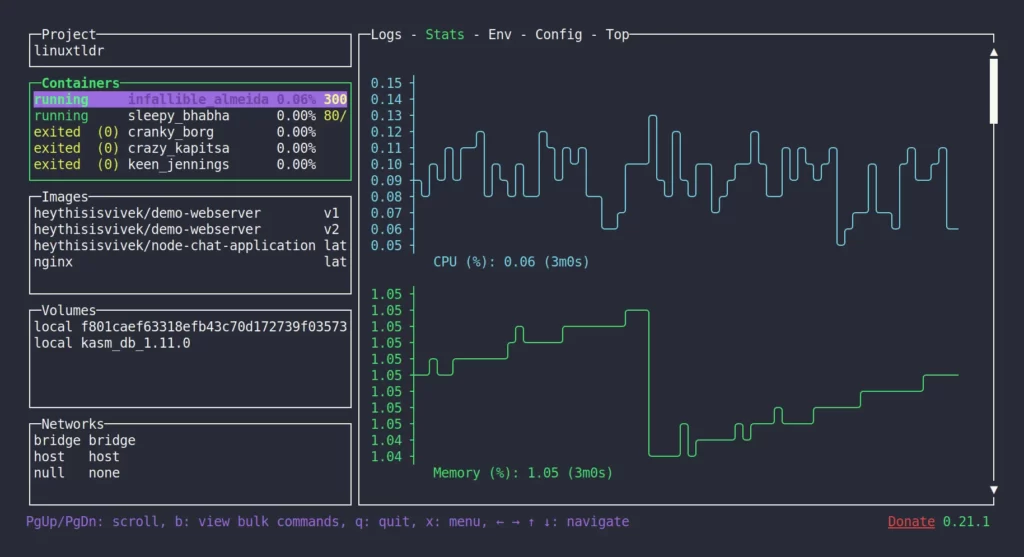
\includegraphics[width=.9\linewidth]{imgs/LazyDocker.png}
    \caption{LazyDocker main screen}
    \label{fig:enter-label}
\end{figure}

\textbf{Dolphie}: A utility for SQL database analytics

\begin{figure}[htbp]
    \centering
    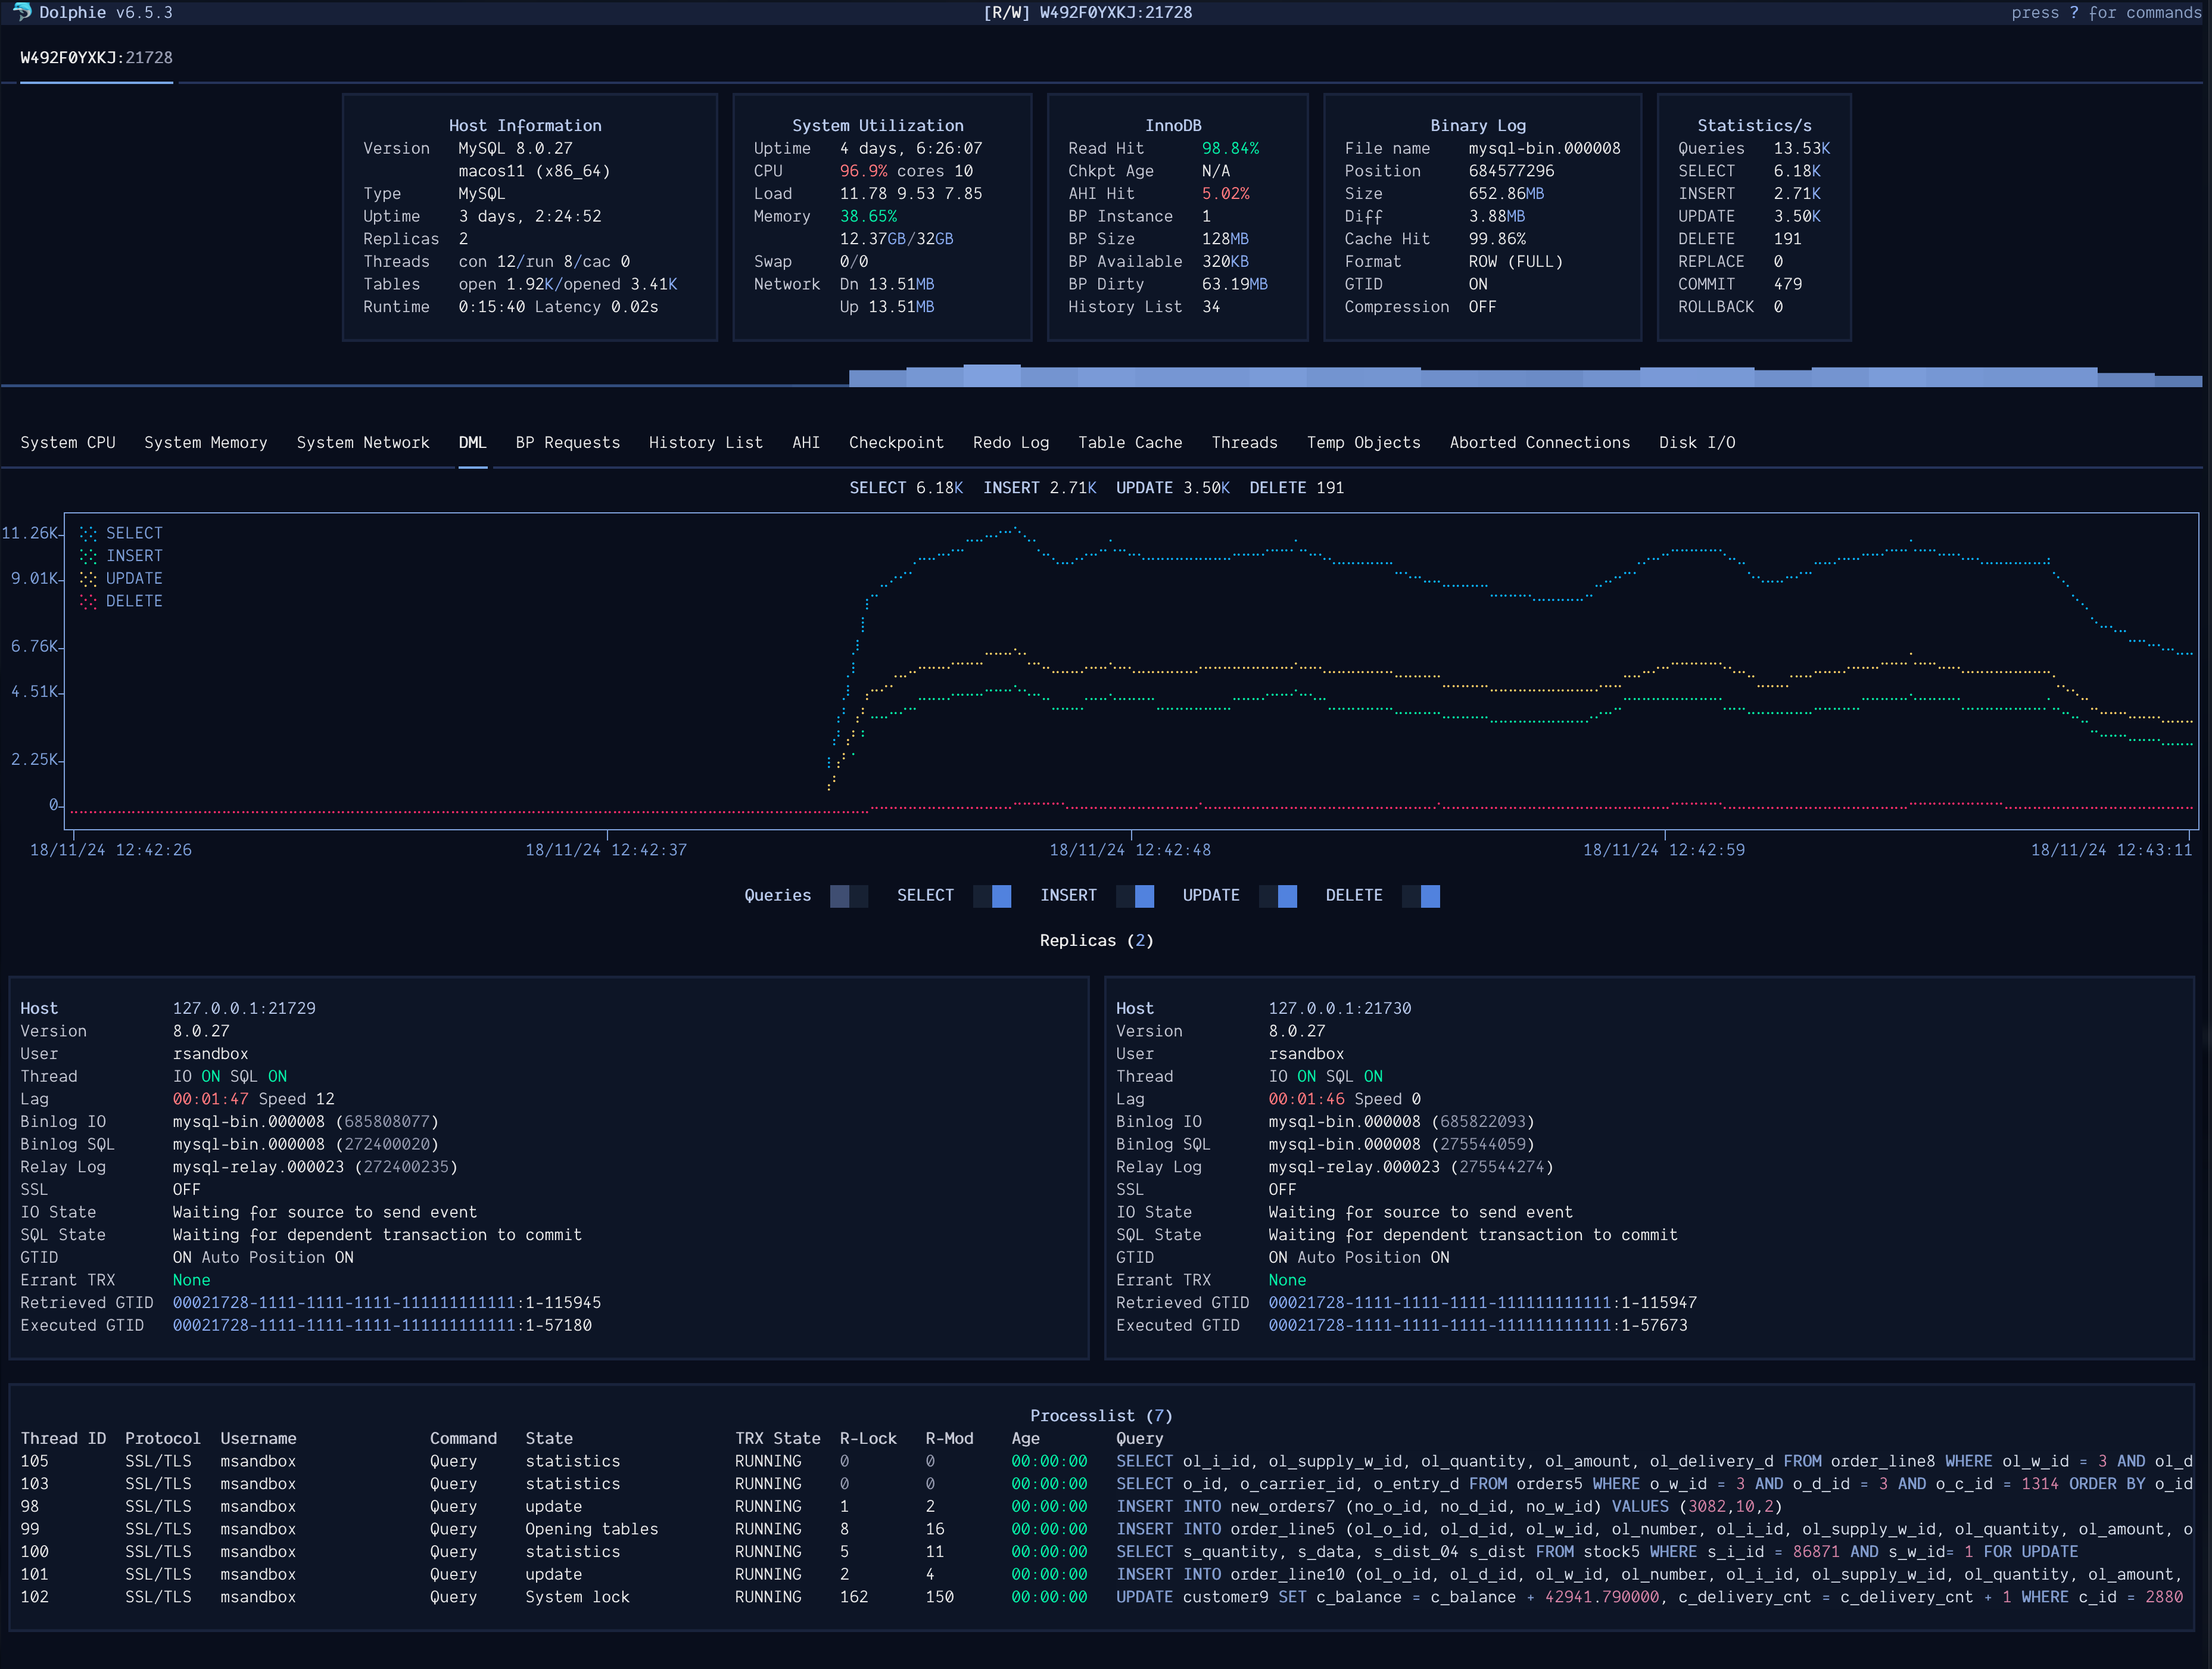
\includegraphics[width=.7\linewidth]{imgs/Dolphie.png}
    \caption{Dolphie main screen}
    \label{fig:enter-label}
\end{figure}

These are tools I personally use daily and find convenient. They allow me to quickly access necessary information. 

\subsection{LazyDocker Analysis}\label{subsec:ld_analysis}

To understand how exactly these tooks work, I analyzed LazyDocker.

\begin{figure}[htbp]
    \centering
    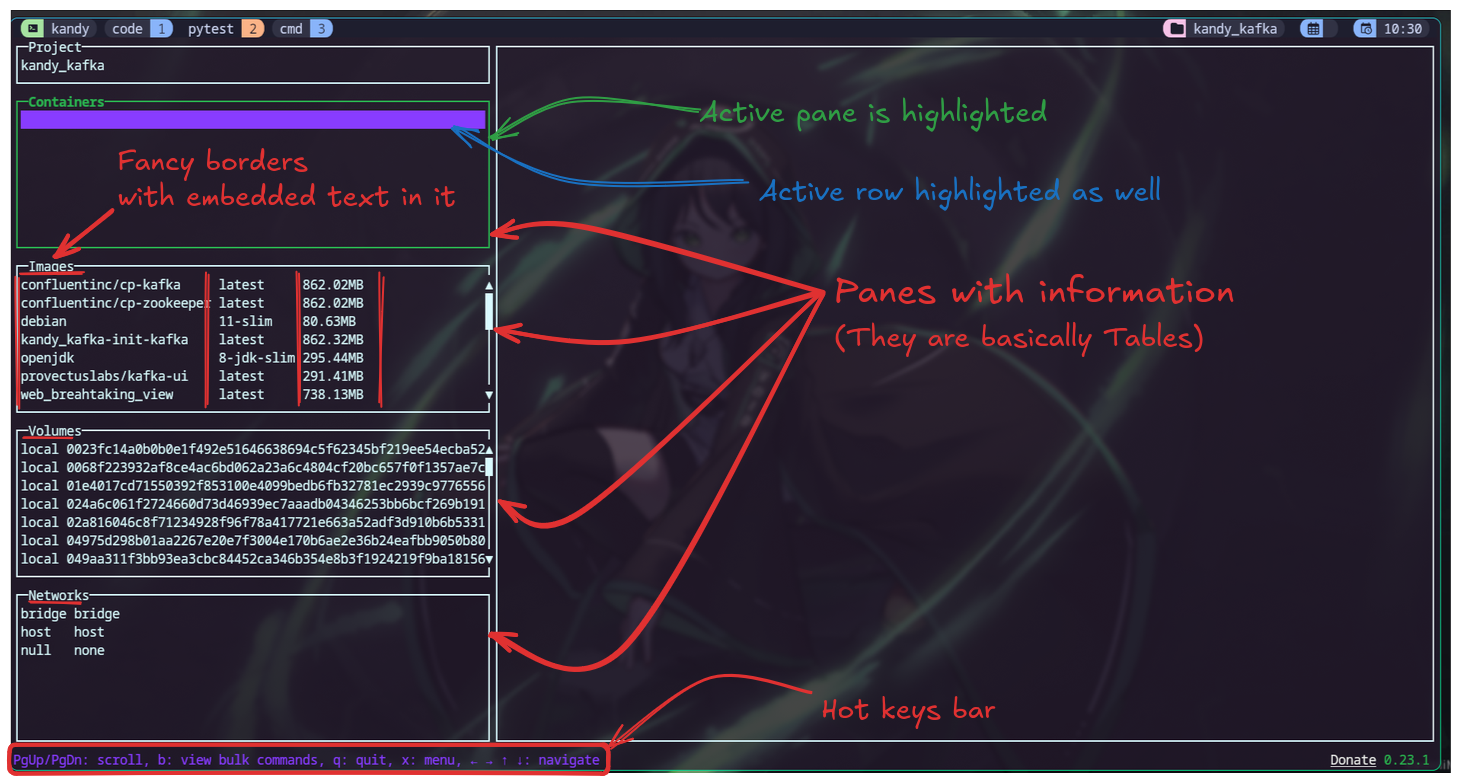
\includegraphics[width=.9\linewidth]{imgs/LazyDockerAnalysis.png}
    \caption{Lazydocker main screen analysis}
    \label{fig:lazydocker_analysis}
\end{figure}

When launching the utility, we can see the compact and minimalist design. All necessary categories are divided into panes, and navigation between them is performed by pressing \texttt{Tab}/\texttt{Shift+Tab} or using arrow keys. At the bottom of the screen, there’s also a bar with shortcut keys.

Panes are the most critical component of this interface. They display information, and their layout heavily influences the user experience. In the case of LazyDocker, the panes work as tables or lists of options. Beyond names, they show essential information, allowing users to navigate without guessing and compare container performance without opening detailed logs.

Additionally, there’s one large pane with detailed information about the selected container/image or network. This pane occupies more than half the screen, providing ample space for detailed data.

\begin{figure}[htbp]
    \centering
    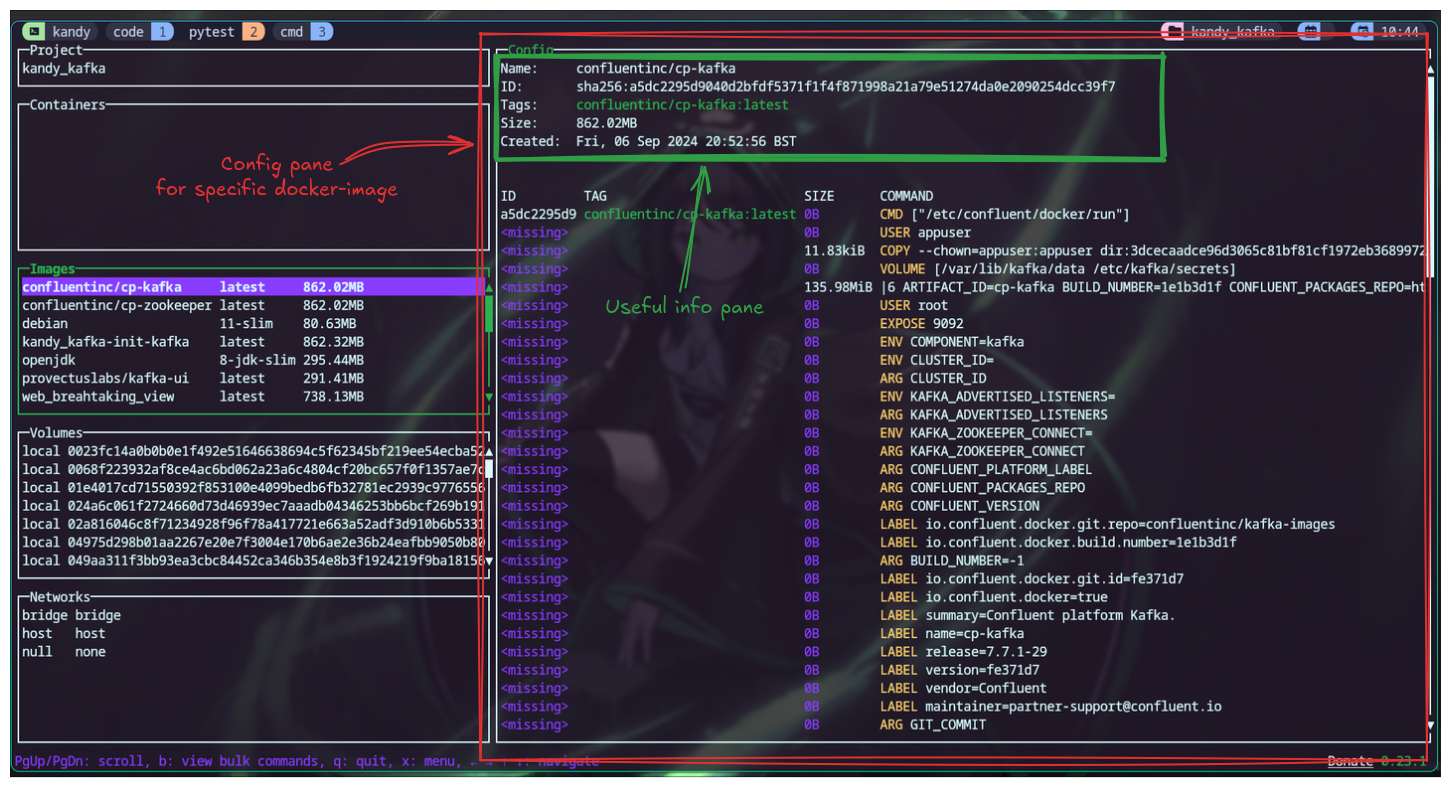
\includegraphics[width=.9\linewidth]{imgs/LazyDockerConfigPane.png}
    \caption{LazyDocker: Config pane}
    \label{fig:ld_big_pane}
\end{figure}


This pane is divided into several tabs. Besides configuration tab (\ref{fig:ld_big_pane}), you can view statistics for each container (\ref{fig:ld_stats_screen}), environment variables (\ref{fig:ld_env_pane}), and resource usage (\ref{fig:ld_top_pane}). This pane is the primary and most convenient feature for day-to-day Docker management. I believe a similar approach could be applied to my product.

\begin{figure}[htbp]
\centering
\begin{subfigure}{.5\textwidth}
    \centering
    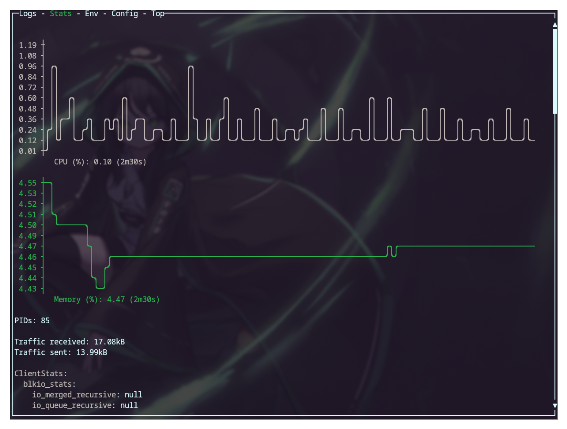
\includegraphics[width=.8\linewidth]{imgs/LazyDockerStatsPane.png}
    \caption{Stats}
    \label{fig:ld_stats_screen}
\end{subfigure}%
\begin{subfigure}{.5\textwidth}
    \centering
    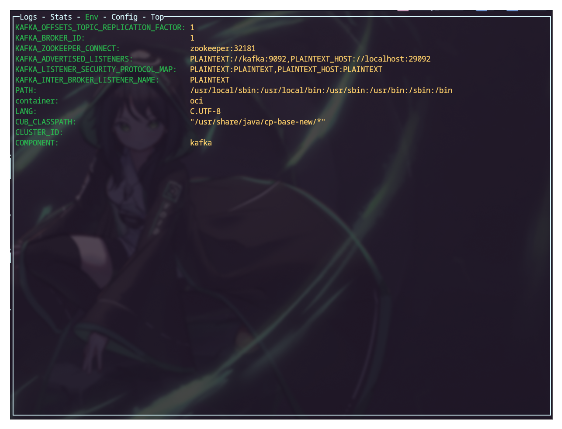
\includegraphics[width=.8\linewidth]{imgs/LazyDockerEnv.png}
    \caption{Env}
    \label{fig:ld_env_pane}
\end{subfigure}

\begin{subfigure}{.5\textwidth}
    \centering
    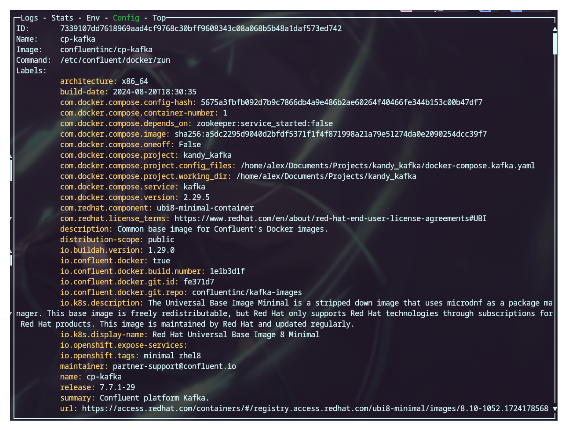
\includegraphics[width=.8\linewidth]{imgs/LazyDockerConfig.png}
    \caption{Config}
    \label{fig:ld_config_pane}
\end{subfigure}%
\begin{subfigure}{.5\textwidth}
    \centering
    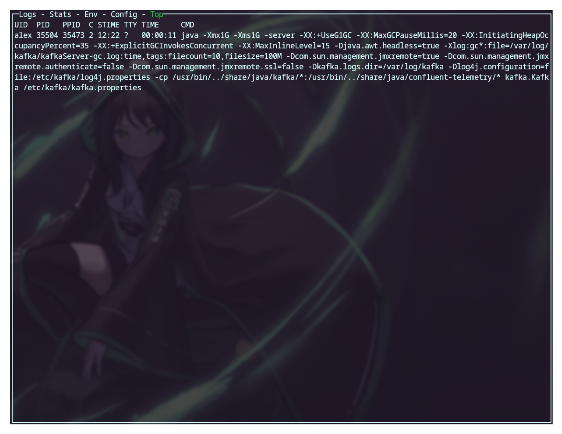
\includegraphics[width=.8\linewidth]{imgs/LazyDockerTopPane.png}
    \caption{Top}
    \label{fig:ld_top_pane}
\end{subfigure}
\caption{Big pane tabs}
\end{figure}

\begin{figure}[htbp]
    \centering
    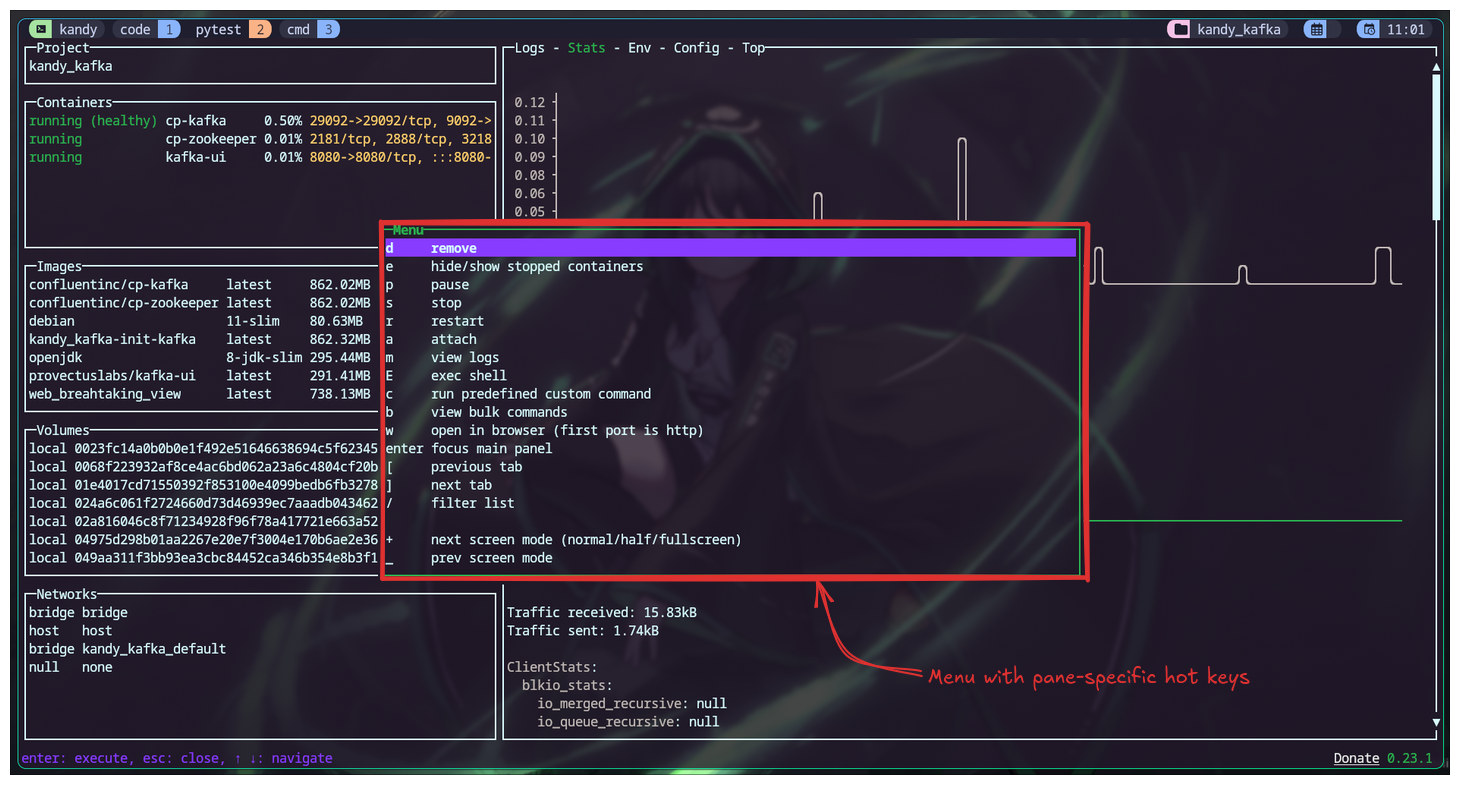
\includegraphics[width=.9\linewidth]{imgs/LazyDockerHotKeysMenu.png}
    \caption{Hotkey Menu}
    \label{fig:enter-label}
\end{figure}

Lastly, pressing a hotkey \texttt{X} opens a menu with a wide range of commands. Hotkeys are designed to speed up processes, and this kind of menu, which consolidates all necessary commands, significantly enhances efficiency. Unlike the bar, this menu allows for a detailed description of each key binding.

This is probably my favorite feature of LazyDocker because it eliminates the need to exit the utility and type lengthy commands to accomplish simple tasks and basiclly speeds up my work several times. I definitely plan to implement such a menu in my product.


\subsection{Conclusions}

After analyzing LazyDocker, I identified key features that could be useful in creating my own utility:

\begin{itemize}
    \item \textbf{Pane-based layout}: This structure looks harmonious and logical for such utilities. Each pane functions as a container, simplifying the logic of information display.
    \item \textbf{Table-like panes}: Displaying data in this format aligns with Kafka’s structure and is likely the optimal solution.
    \item \textbf{Menu and hotkey bar}: These elements make navigation through the interface a quick and effortless task, often requiring no conscious thought.
    \item \textbf{Tabbed panes}: As with the large pane, using tabs instead of separate screens can sometimes be more convenient and logical.
    \item \textbf{Colors}: Though not explicitly mentioned earlier, colors play a vital role both aesthetically and functionally. Highlighting the active pane, using a “traffic light” system to display container statuses, and syntax highlighting for configurations all enhance the user experience.
\end{itemize}

By incorporating these features, I aim to develop a TUI application that is both efficient and user-friendly.

\newpage
\section{Features of the proposed solution}
\label{sec:proposed_features}
\begin{figure}[htbp]
    \centering
    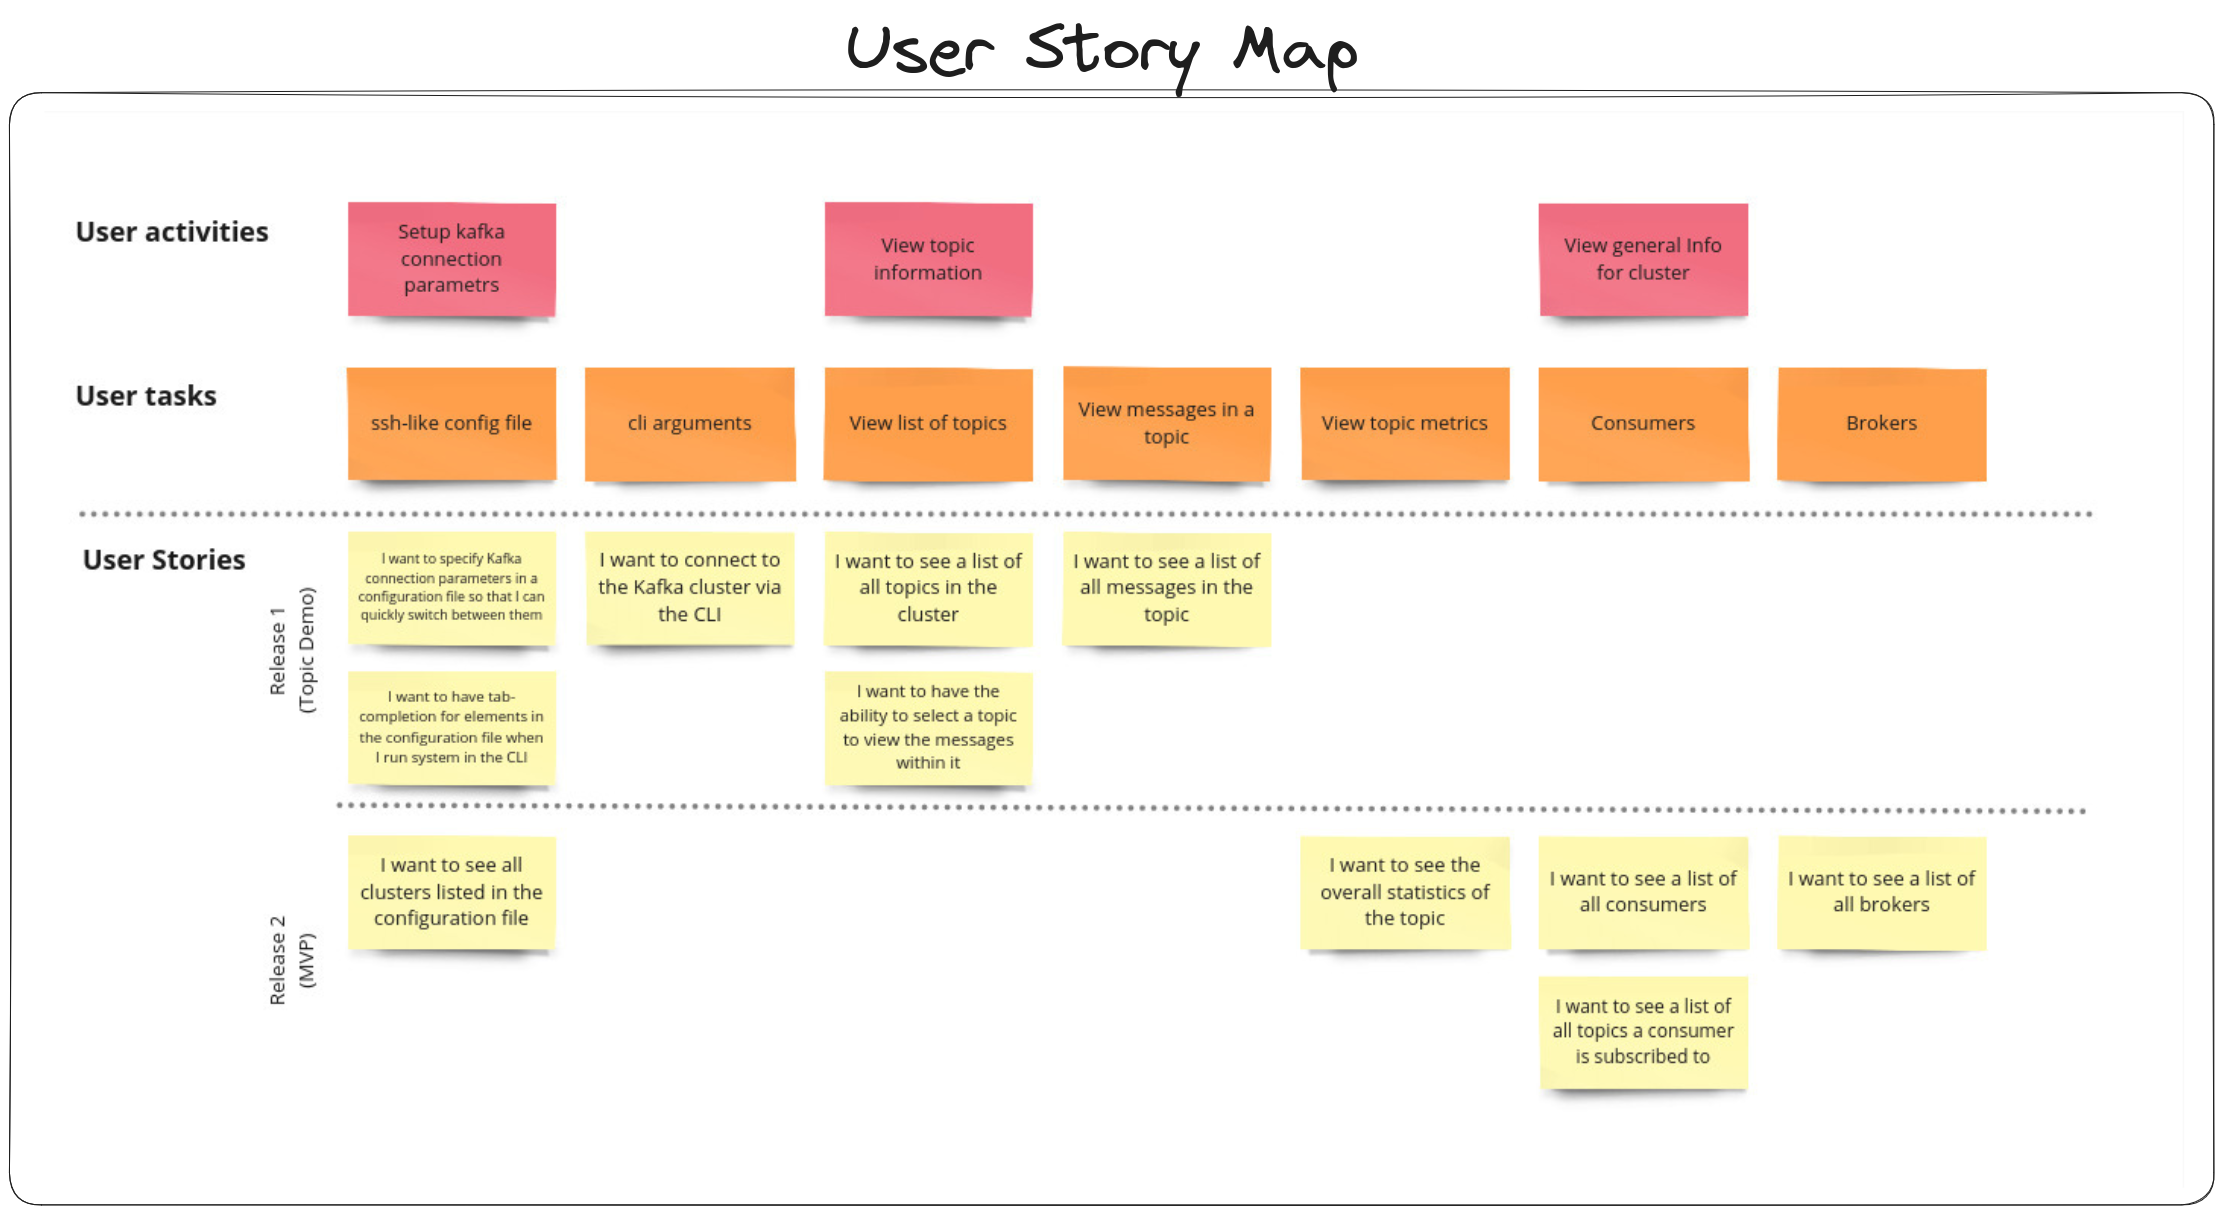
\includegraphics[width=1\linewidth]{imgs/UserStoryMap.png}
    \label{fig:USM}
\end{figure}

To outline the initial application concept and plan for future development, I chose to use User Story Mapping (USM). This approach provides a user-centered perspective, aiding in prioritizing features across different development phases. USM is an agile approach to requirements engineering, composed of several key elements:

\begin{enumerate} \item \textbf{User Activity:} This step involves identifying the main activities users will perform within the system, representing the core actions they take to achieve their goals. \item \textbf{User Tasks:} Within each user activity, specific tasks are defined. These tasks represent the necessary steps users must follow to accomplish the activity. \item \textbf{User Stories:} Each task is further refined into user stories. These stories represent the functionalities or features needed to fulfill the task from the user's perspective. \end{enumerate}

In a User Story Map, user stories are organized into swimlanes based on their release phases. Releases indicate the prioritization of user stories, outlining which ones should be completed first. The essential structure of USM lies in its sequential arrangement of user tasks from left to right, aiming to provide a comprehensive overview of user interactions with the system. This format helps ensure a clear understanding of user needs and workflows.

One of the main advantages of USM over other requirements engineering techniques is its flexibility to accommodate changes based on user feedback. Its visual representation also aids in understanding the system from the user’s perspective, enhancing communication and collaboration among stakeholders.

On the map, tasks are divided into two releases: Topic Demo and MVP. The Topic Demo represents the initial stage, where I will create the application framework, TUI, and add the essential topic-viewing feature. This demo serves as a basis for consulting with my stakeholder and allows for adjustments to the USM if needed.

After consulting with Sarah, I will refine the application according to her feedback and proceed to work on the second release, MVP (Minimal Viable Product). This release will include additional features, such as displaying statistics across all topics and enabling interaction with consumer groups.

\section{Limitations of my solution:}

The primary limitation of this solution is time. As this project is part of the A-level coursework, alongside other assignments, my task estimates may be overly optimistic. Working independently, I may realistically only be able to implement a portion of the planned functionality.

Additionally, there are limitations associated with the libraries I intend to use. Currently, I am considering urwid or textual for developing the TUI (Text User Interface). However, urwid, for instance, does not support a broad range of terminal types and may perform inconsistently in certain environments, which could pose challenges and restrict my solution’s effectiveness.

\chapter{Requirements}

\section{Software product quality model}

\begin{figure}[htbp]
    \centering
    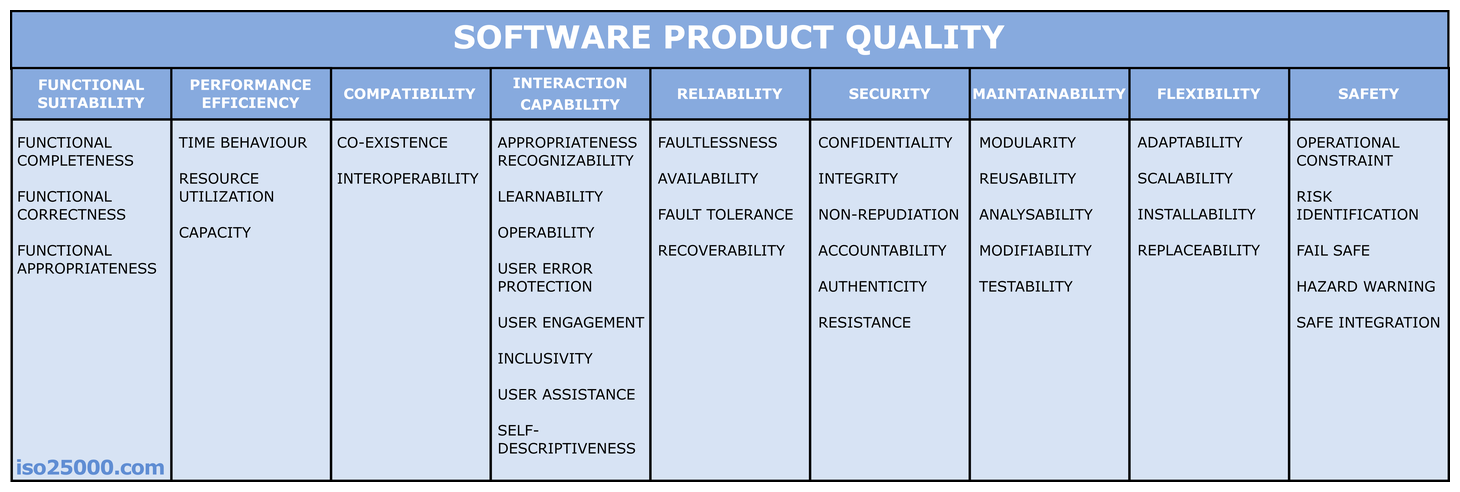
\includegraphics[width=1\linewidth]{imgs/ISO25010.png}
    \label{fig:quality_model}
\end{figure}

    I based my quality requirements on the ISO 25010 standard, which outlines the key characteristics of any software product, and developed a quality model using the QAS (Quality Attribute Scenarios) methodology. To achieve this, I identified critical attributes by referencing both interviews with Sarah and industry standards. A description of the model and its attributes is provided below.
    
\newpage

\subsection{Quality Attribute Scenarios (QAS)}

Each quality attribute is defined through quality attribute scen-arios, which must adhere to the six-part rule. For more information on this method, see https://wstomv.win.tue.nl/edu/2ii45/year-0910/Software\_Architecture\_in\_Practice\_2nd\_Edition\_Chapter4.pdf

\begin{table}[h!]
    \centering
    \renewcommand{\arraystretch}{1.3} % Set a comfortable line spacing
    \begin{adjustbox}{max width=\textwidth} % Fit table to page width
        \begin{tabular}{| p{3.5cm} | p{10.5cm} |}
            \hline
            \textbf{Term} & \textbf{Description} \\ \hline
            Stimulus & Describes an event arriving at the system, like a performance event, user operation, or security attack. A stimulus for modifiability could be a modification request, while for testability, it could be a phase completion. \\ \hline
            Stimulus Source & The origin of a stimulus, affecting how the system treats it. For example, a trusted user’s request may be handled differently from an untrusted user's. \\ \hline
            Response & Specifies how the system or developers should act in response to the stimulus, detailing responsibilities at runtime or during development. \\ \hline
            Response Measure & Defines how to judge if the response meets requirements, helping determine if the system or developer actions are sufficient. \\ \hline
            Environment & The context in which the scenario occurs, which qualifies the stimulus and influences system response. \\ \hline
            Artefact & The part of the system to which the requirement applies, often the entire system but sometimes only specific components. \\ \hline
        \end{tabular}
    \end{adjustbox}
    \caption{Definitions of Key Terms}
\end{table}

\subsection{Environment}
    I am gonna use my laptop as a \textbf{normal operating conditions} for several reasons. First of all, it's always at hand, so I don't need to worry about logistics or where I'll be testing the product. Secondly, I have a fairly average laptop in terms of specifications, so if the utility works smoothly on it, it will likely work on more powerful machines as well. Therefore, all hardware requirements are based on the basic characteristics of my device and all software requirements are based on the installed software on the my machine.

\begin{table}[h!tbp]
\centering
\begin{tabular}{| l | l |}
\hline
\textbf{Part of environment} & \textbf{Variable} \\
\hline
OS & Manjaro Linux 23.1.4 (Vulcan) \\
\hline
Terminal Emulator & Kitty 0.31.0 \\
\hline
Kafka version & confluentinc/cp-kafka:7.7.1\\
\hline
Python version & 3.11.4 \\
\hline
CPU & 1.60 GHz \\
\hline
RAM & 4 GB \\
\hline
Docker version & 25.0.3 \\
\hline
Python libs versions & Specified in the file \textbf{pyproject.toml} in~Appendix:\ref{appendix:libs} \\
\hline

\end{tabular}

\end{table}
As Kafka will be deployed on the same system where Kandy is tested, I anticipate virtually negligible latency when it comes to communicating between services


\newpage
\section{Success criteria}
\begin{table}[h!tbp]
\centering

\begin{tabular}{|p{7cm}|p{5cm}|p{3cm}|}
\hline
\textbf{Criteria} &  Justification&Evidence \\
\hline
Time behaviour QAS have passed successfully (Response time less than 10 seconds https://www.nngroup.com/articles/response-times-3-important-limits/)&  &.log file \\
\hline
 &   &\\
\hline
 &   &\\
\hline

\end{tabular}

\end{table}

\chapter{Design}

Having identified the requirements and success criteria, I can now proceed with designing the system itself. The primary goal of this process is to create a structure that facilitates the addition of new features and the maintenance of the project while preserving or improving its functionality. A thoughtful design approach is essential to ensure effective system development, maintainability, scalability, and adaptability for future changes.

Any design process begins with the decomposition of the problem into manageable pieces of work and domain-specific elements. This activity often involves brainstorming. As a visual thinker, I decided to create a diagram that depicts the elements and sections of the system being designed.

\section{Decomposition}

The first level of elements I identified is as follows:
\begin{itemize}
    \item Define core functional requirements
    \item Choose development technology
    \item Design user interface structure
    \item Test and debug
    \item Release and support
\end{itemize}

Since I am building a tool for an existing software system, my tool is heavily dependent on its core functionality and capabilities. Therefore, understanding and defining the core functional requirements is a high-priority activity.

Choosing suitable development technology is critical for several reasons. First, it must enable technical integration with Kafka. Second, I must have sufficient expertise in the chosen technology to ensure that the project is completed within the set timeline.

Given that the project goal is to create an application with a user interface (UI) to enhance how target users interact with Kafka, I need to carefully plan the UI's structure and design to ensure an optimal user experience.

Any software application requires an appropriate level of testing. To define what ``appropriate'' means for my application, I must consider how the system will be tested and determine the level of logging required to ensure that it works as expected.

The final phase of application development involves delivering the software to the target users. The process of installation and running the application is just as important as the application requirements themselves. Thus, I aim to plan ahead and identify the tools and strategies needed to make this process as seamless as possible.

In the following sections, I will explain my thought process for each element and how they contribute to the system's development.

\newpage

\subsection{Legend}

\begin{figure}[htbp]
    \centering
    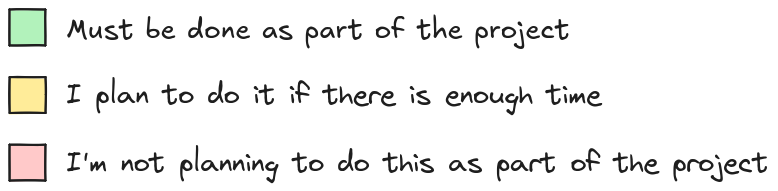
\includegraphics[width=.6\linewidth]{imgs/DesignLegend.png}
    \caption{System Design Diagram Legend}
    \label{fig:design_legend}
\end{figure}

In \textbf{Figure~\ref{fig:design_legend}}, the system design diagram legend provides a key for understanding the system design diagram. It is applicable for all the following diagrams in this section. 

For the full diagram, refer to \textbf{Appendix~\ref{appendix:system_design}}. Given the large size of the diagram, I will discuss its components and subdivisions separately in the following sections

\subsection{Define core functional requirements}

As mentioned earlier, understanding and defining the core functional requirements is a high-priority activity. I have divided this into three main blocks:

\begin{figure}[htbp]
    \centering
    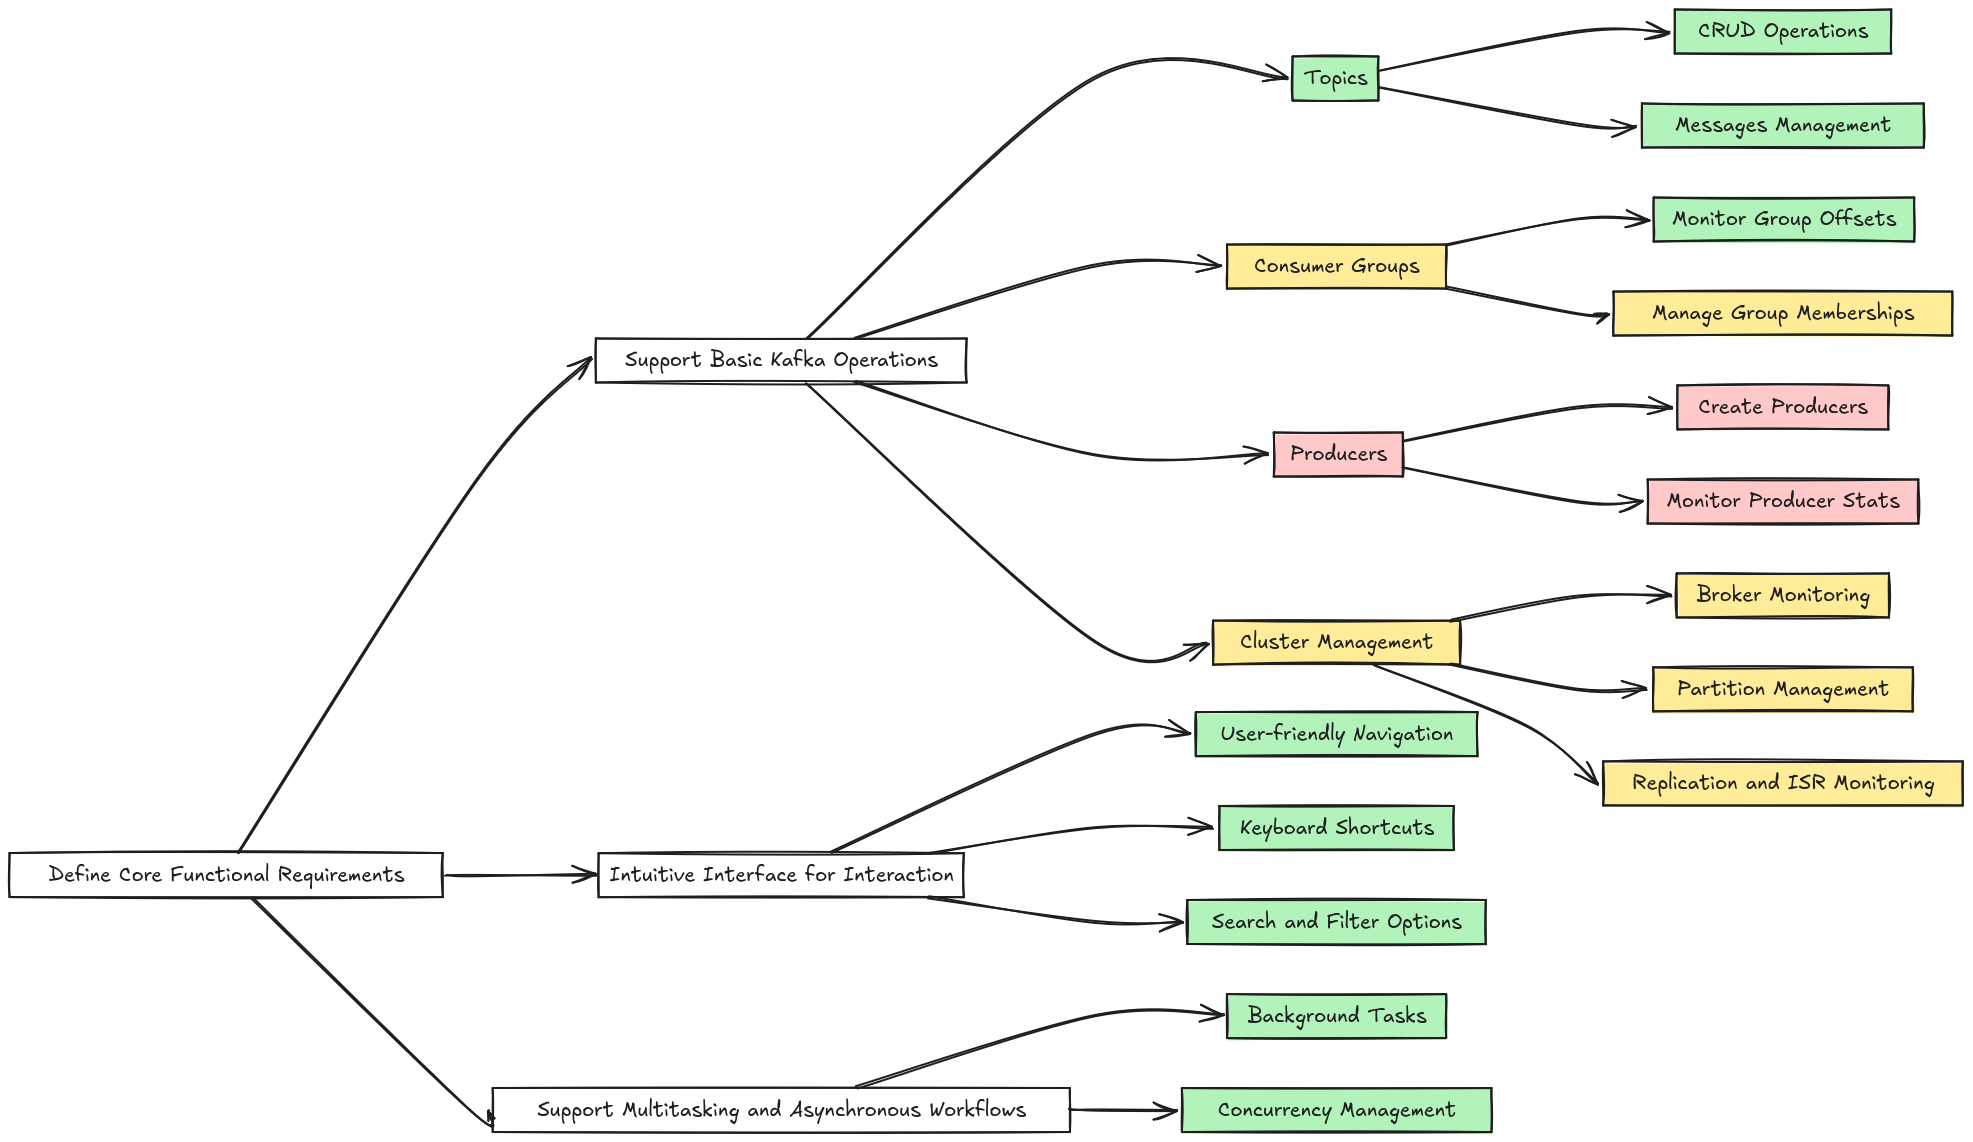
\includegraphics[width=1\linewidth]{imgs/CoreFucntionalRequirementsDiagram.png}
    \caption{Core Functional Requirements}
    \label{fig:core_functional_requirements}
\end{figure}

\begin{itemize}
    \item \textbf{Basic Kafka Operations} — This involves core functionalities for interacting with Kafka. These are features that are essential for any Kafka management utility. I have outlined them separately in Figure~\ref{fig:basic_kafka_operations}, which I will discuss further below.
    
    \item \textbf{Intuitive Interface} — Since I am developing a terminal-based utility for developers who are accustomed to working with terminal applications like Vim, creating user-friendly navigation through versatile keyboard shortcuts is a priority. Additionally, because Kafka is inherently designed for processing large volumes of data, it is essential to provide users with the ability to quickly search for relevant information within a large data stream.
    
    \item \textbf{Multitasking and Asynchronous Workflows} — Again, considering Kafka’s nature of handling significant amounts of data, the fetching process can take time. Ensuring concurrency of processes in this scenario is necessary, and implementing background tasks will be an effective solution.
\end{itemize}

\begin{figure}[htbp]
    \centering
    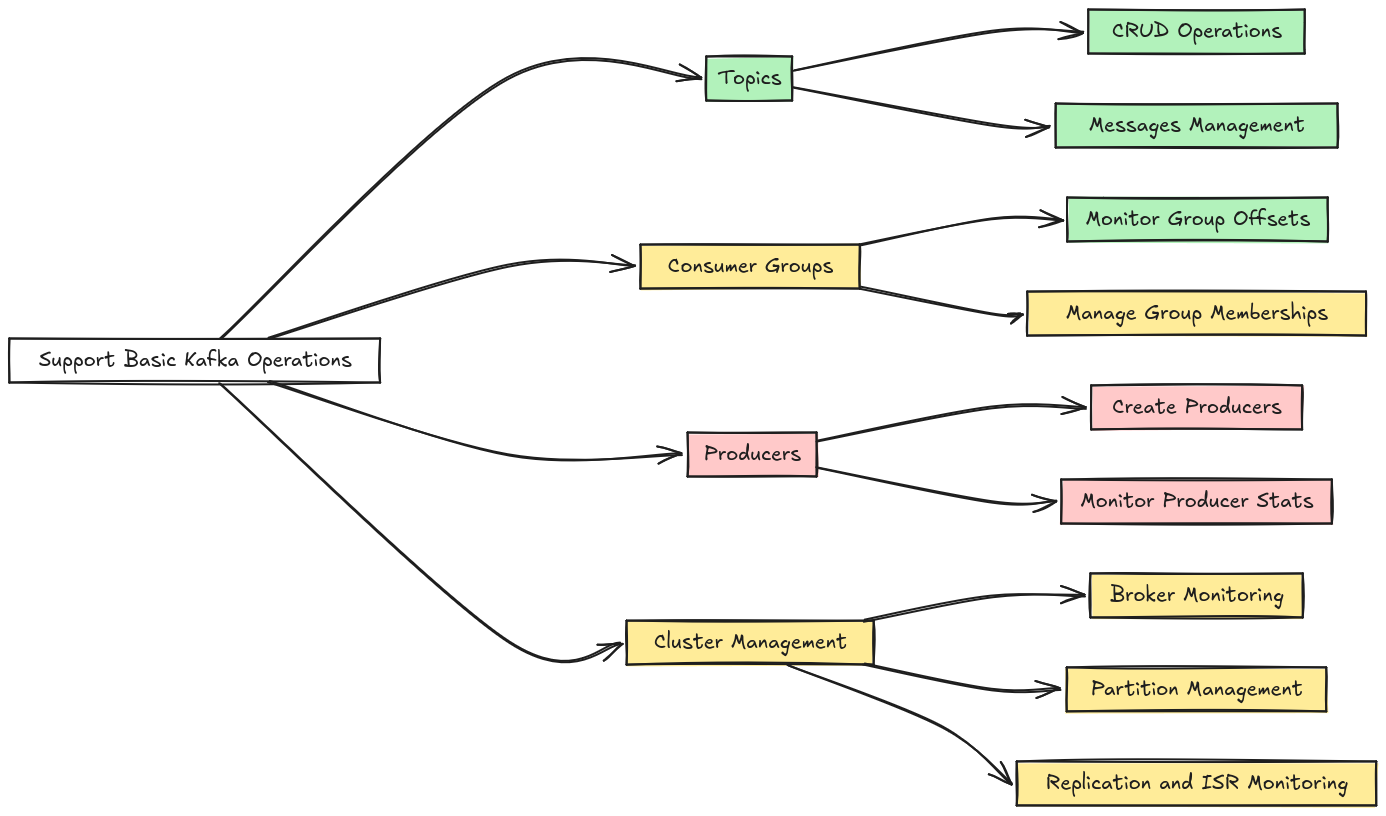
\includegraphics[width=1\linewidth]{imgs/BasicKafkaOperationsDiagram.png}
    \caption{Basic Kafka operations requirements}
    \label{fig:basic_kafka_operations}
\end{figure}

\section{Design}

\begin{figure}[htbp]
    \centering
    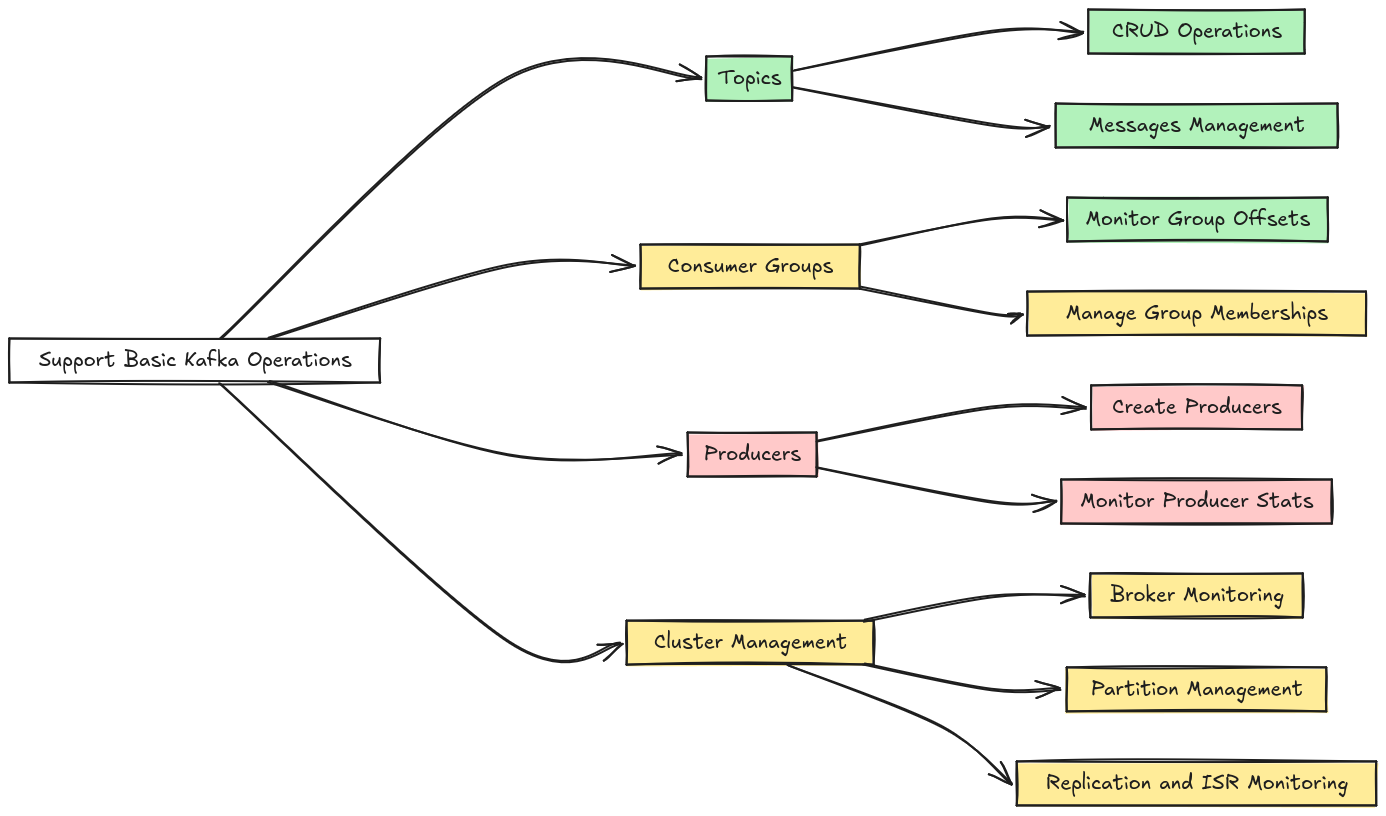
\includegraphics[width=1\linewidth]{imgs/BasicKafkaOperationsDiagram.png}
    \caption{Basic Kafka operations requirements}
    \label{fig:basic_kafka_operations}
\end{figure}

Based on Kafka's basic architecture (Figure~\ref{fig:kafka_arch}), four primary features come to mind that the management utility must support:
\begin{itemize}
    \item Working with topics
    \item Managing consumer groups
    \item Interfacing with producers
    \item Cluster management
\end{itemize}

The project is significantly constrained by time, so I divided tasks into three categories (Figure~\ref{fig:design_legend}). 

\textbf{Green}: For the initial release, I must include support for working with topics, specifically creating and deleting them. Additionally, topic management includes reading messages from them. This will be the core functionality of my MVP solution.

\textbf{Yellow}: If time permits, I will work on consumer group management. This feature was highlighted by my stakeholder as useful, but since other interfaces do not support it, it is not essential.

\textbf{Red}: Tasks like cluster management are large in scope, and for the MVP, they would be overkill. I will not include them in this project but will prioritize them for future updates after the initial release.

\subsection{Interface Structure}

\begin{figure}[htbp]
    \centering
    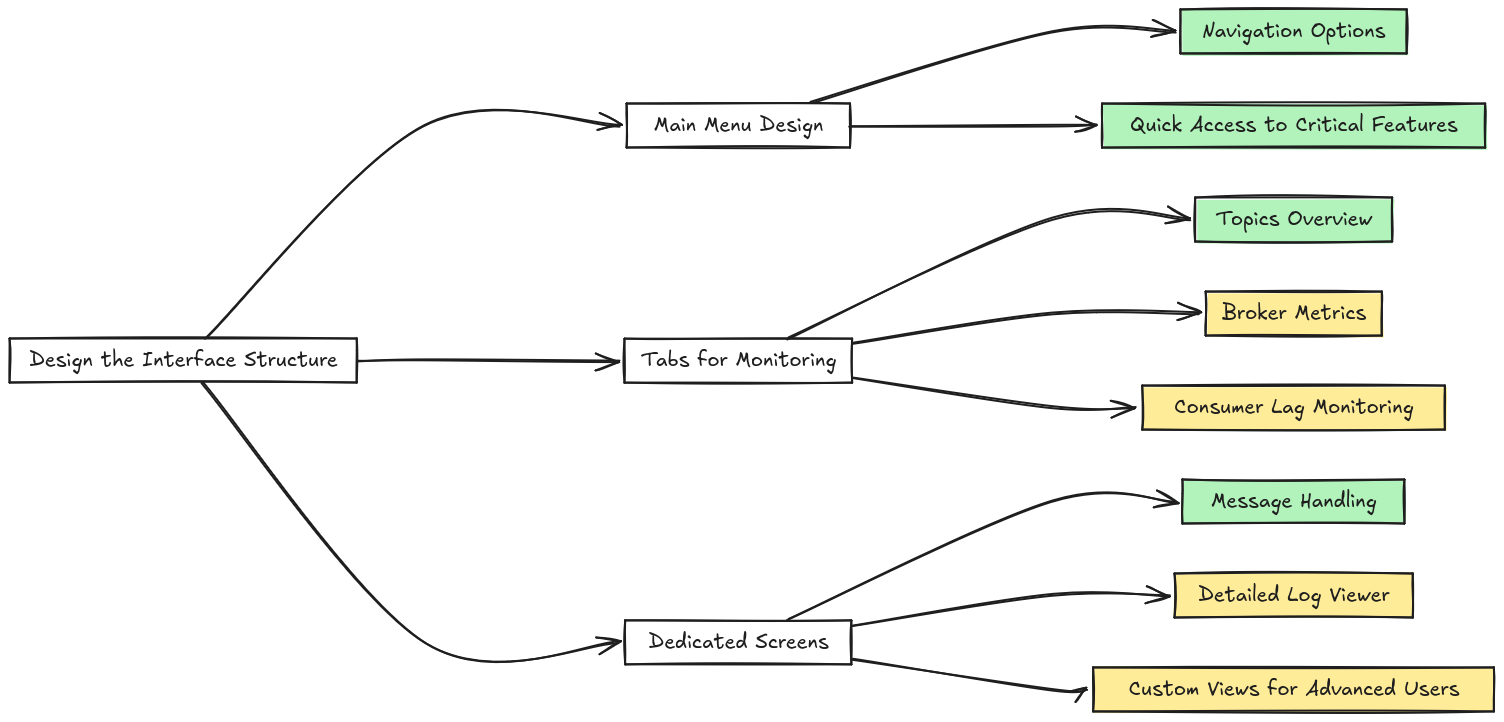
\includegraphics[width=1\linewidth]{imgs/InterfaceDesign.png}
    \caption{Interface design structure}
    \label{fig:interface_design}
\end{figure}

The technologies chosen for UI development significantly influence the design process. Therefore, I want to finalize the interface design before selecting the technology stack. In Figure~\ref{fig:interface_design}, I have highlighted the priority tasks. The most critical aspect is the main menu design, as its navigational capabilities and quick access to core features will determine whether users find the application useful. No matter how powerful the system is, if it’s inconvenient to use, users won’t engage with it.

\subsection{Main Menu Design}

From my analysis of LazyDocker in Section~\ref{subsec:ld_analysis}, I identified several features I would like to include in my solution.

Here, I adapt them to suit the needs of my utility:
\begin{itemize}
    \item \textbf{Panes}: Kafka data is naturally suited for display in table format, as most elements can be easily categorized.
    \item \textbf{Hotkeys}: Hotkeys are what make navigation satisfying. They are essential for any TUI utility. I plan to implement a general hotkeys bar and context-specific menus for individual panes. For example, sorting topics by different parameters can be performed using hotkeys.
    \item \textbf{Navigation}: Navigation is equally important. Moving between panes should be intuitive and straightforward. I decided to support navigation not only with \texttt{Tab}/\texttt{Shift+Tab} and arrow keys but also with vim-style hotkeys. Many developers use vim/emacs plugins in their workflows, and it’s enjoyable to have familiar keybindings across the developer environment.
    \item \textbf{Colors}: As mentioned in the analysis, colors play both an aesthetic and functional role. They help highlight important elements and focus the user’s attention where needed. Ideally, I would like to provide customizable palettes, but for the MVP, I will hardcode a basic color palette. If time permits, I will later update it to be configurable.
\end{itemize}

Based on LazyDocker, I sketched the following main menu mockup:

\begin{figure}[htbp]
    \centering
    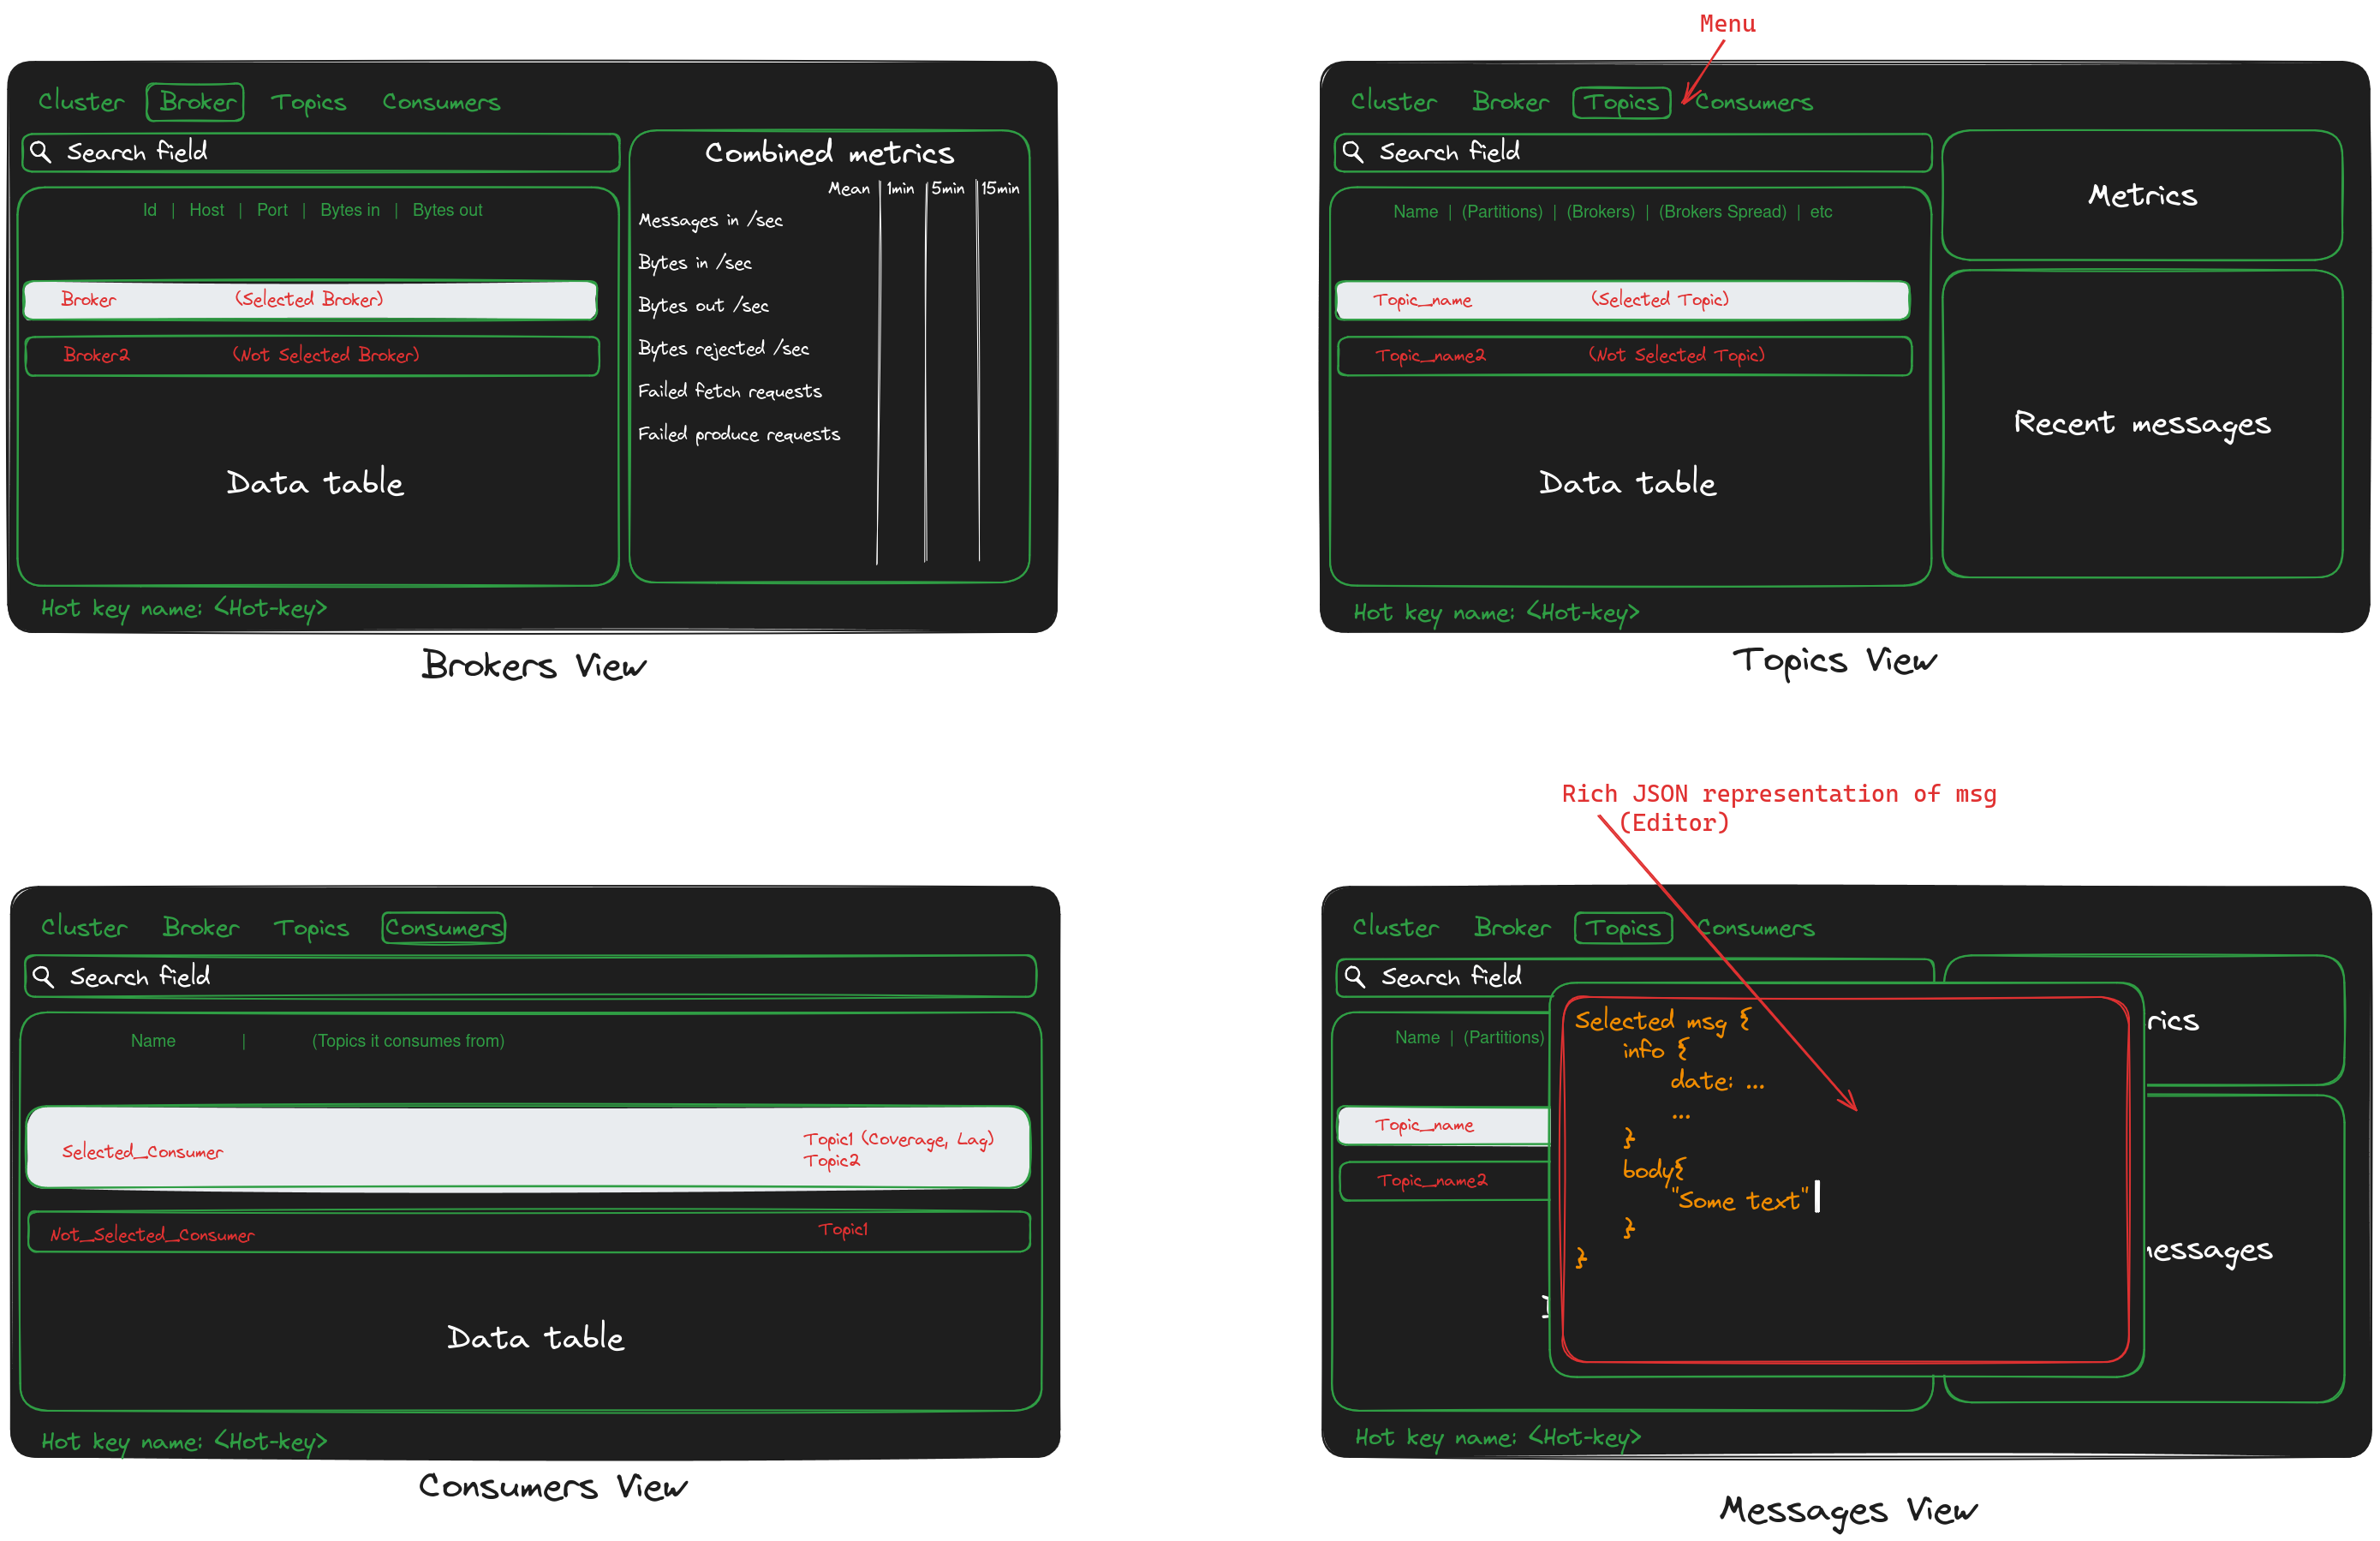
\includegraphics[width=1\linewidth]{imgs/UIMaquette.png}
    \caption{Main menu mockup}
    \label{fig:ui_maquette}
\end{figure}

The first MVP version will only include the topic view and message view. I will discuss these in detail below. For now, a brief note on consumer and broker views: when designing mockups, I drew inspiration from Kafka Manager as a free alternative to Conduktor (which was discussed by Sarah). All views include a data table with various columns. For consumer groups, an initial implementation could include only group names (IDs) and associated topics. The broker screen is intended to track load metrics, so I divided it into two panels—a table panel with general information about each broker and a detailed information panel for the selected broker. In the future, the second panel could include tabs, such as one for rendering load graphs or displaying data loss statistics. To determine their utility, I will consult with my stakeholder.

\begin{figure}[htbp]
    \centering
    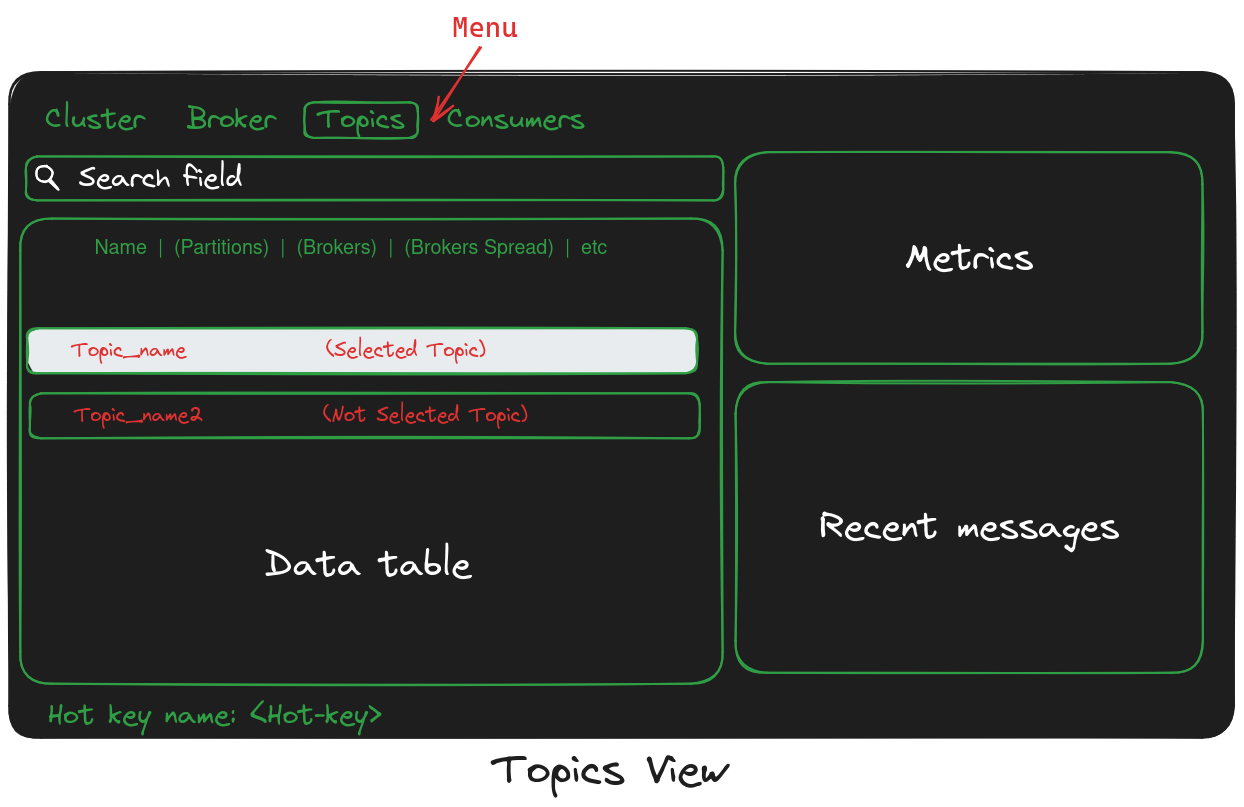
\includegraphics[width=1\linewidth]{imgs/TopicsScreenDesign.png}
    \caption{Topics screen mockup}
    \label{fig:topics_screen_maquette}
\end{figure}

\textbf{Topics View}: This is the main screen users will interact with most frequently, so it will be the first to be implemented for the MVP. This screen is divided into three panes:
\begin{itemize}
    \item A general pane displaying information about topics in the cluster.
    \item A metrics pane for the selected topic, potentially including graphs for specific time periods. Initially, it will display basic data.
    \item A messages pane showing the last \textit{N} messages in the selected topic. By pressing enter on any topc will open new screen with messages stored in this topic (Figure~\ref{fig:message_view}).
\end{itemize}

\begin{figure}[htbp]
    \centering
    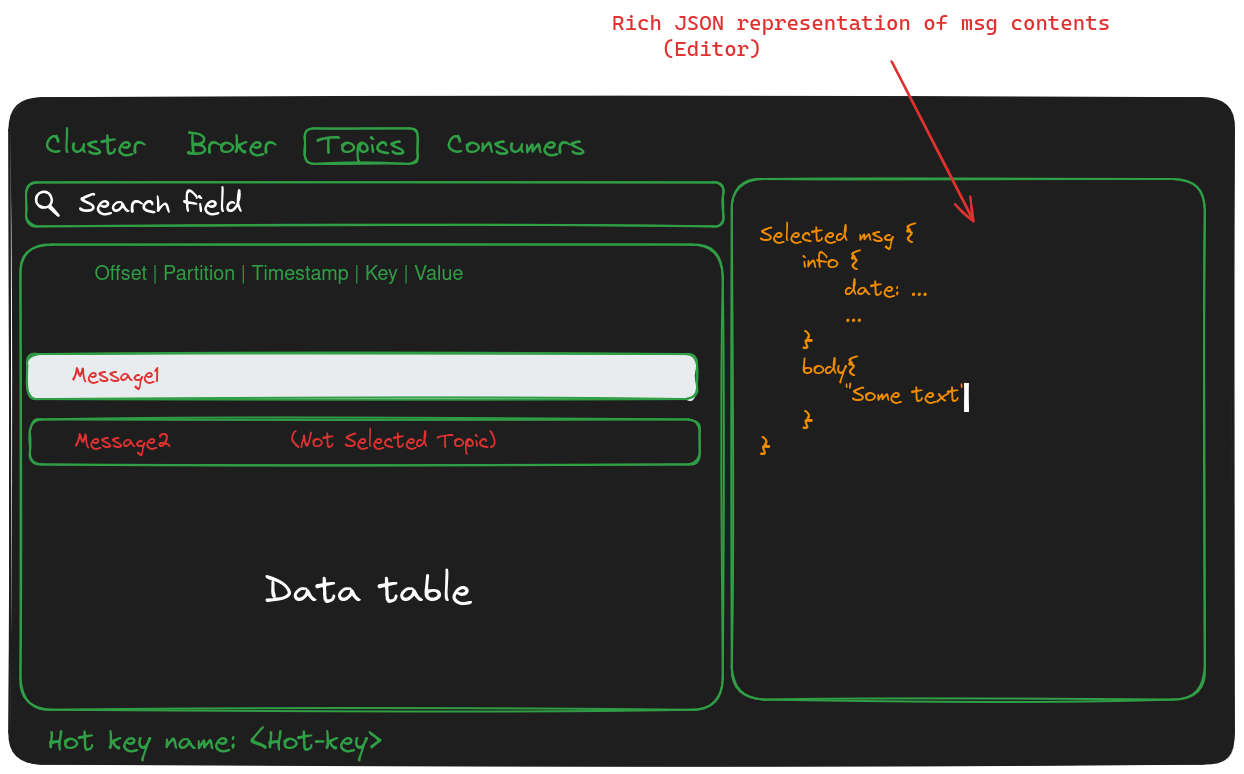
\includegraphics[width=1\linewidth]{imgs/MessageView.png}
    \label{fig:message_view}
    \caption{Message view}
\end{figure}

В целом этот экран не сильно отличается от экрана топиков, он показывает сообщения табличном виде, при выборе сообщения можно посмотреть его содержимое в editore в правой части экрана.

\subsection{Tech Stack}

Определившись с двумя важнейшими частами интерфейса я могу перейти к определению стака технологий, ниже на Figure~\ref{fig:tech_chart} я опять разделил технологии на три составляющие.

\begin{figure}[htbp]
    \centering
    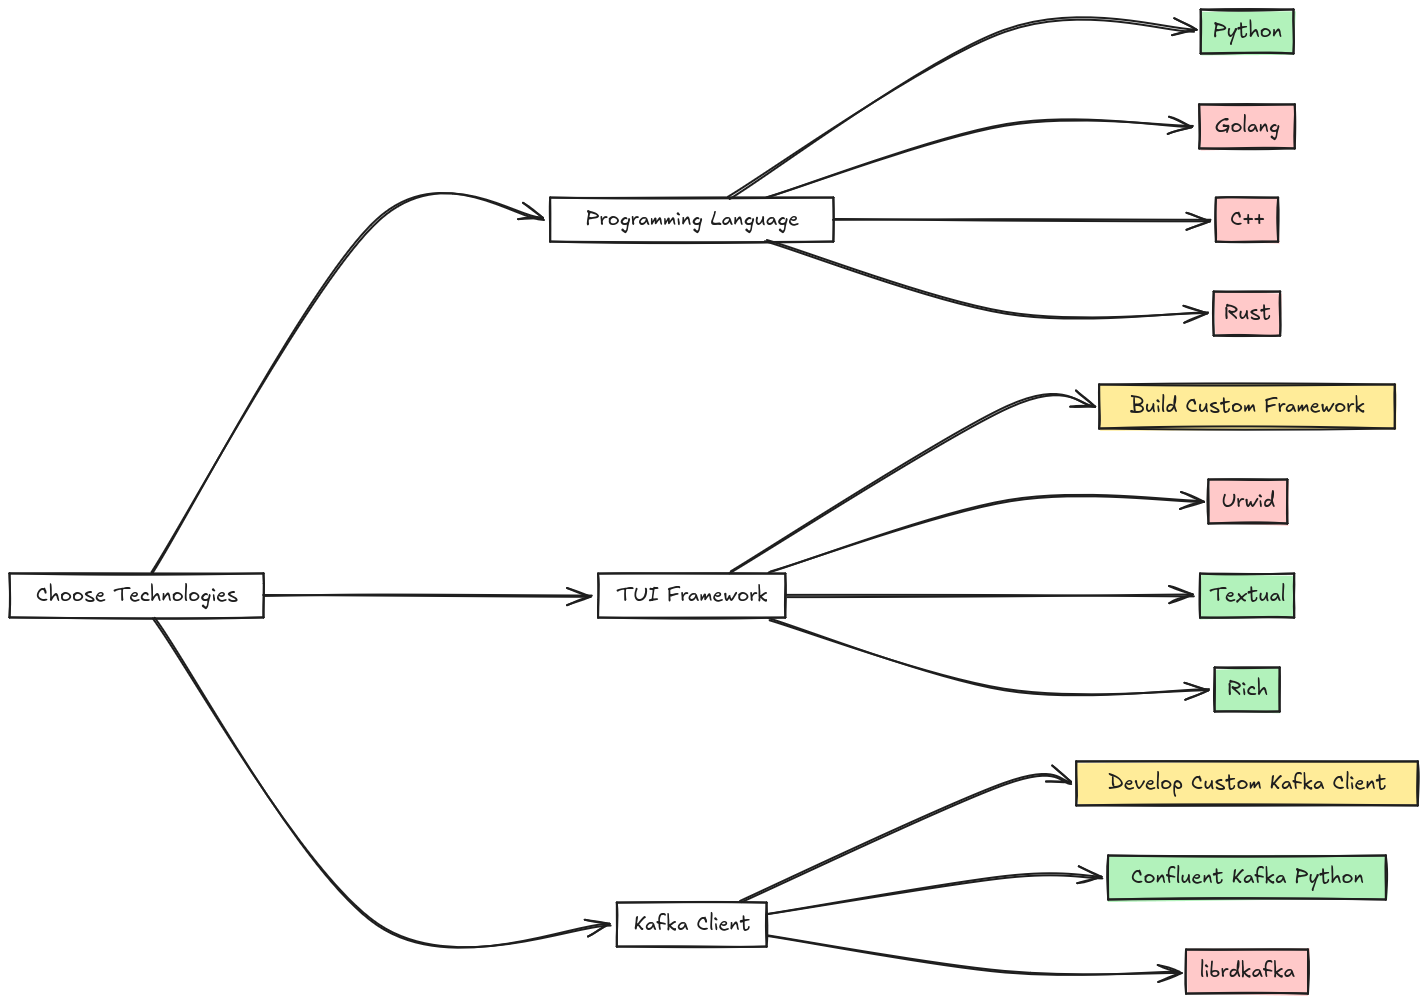
\includegraphics[width=1\linewidth]{imgs/TechDiagram.png}
    \label{fig:tech_chart}
\end{figure}

\textbf{Programming language}: Важнейшее решение для проекта, от языка зависит перформанс, стиль кода и подход к разработке в целом. Я бы наверное использовал rust или go, но к сожалению с ними я не знаком на достаточном уровне, чтобы быть увереным, что я смогу довести проект до какой-либо приемлемой стадии в сжатые сроки. C++ и C попадают в список rejected по той же причине, хотя и являются перспективным выбором, ведь я пишу приложение в оснвном расчитанное на Линуксоидов. Для создания легковесного, оптимизированного интерфейса для линуксовой командной строки эти два языка, мне кажется, подошли бы лучше всего. Я отказался от этих языков в пользу питона. Питон - простой для чтения и в тоже время очень мощный язык, имеет обширную базу библиотек, а еще я с ним занаком с 8 лет, так что я могу достаточно точно оценить многие задачи in terms of time, поэтому он будет лежать в основе проекта. 

\textbf{TUI Framework}: Далее по важности идет именно UI. Проведя ресерч я выделил четыре(На самом деле три) опции. Urwid, относительно устаревшая библиотека с не очень детальной документацией, но по скриншотам выглядит так, будто содержит в себе все нужные блоки и функционал для создания интерфейса по макетам. Из минусов поддерживает всего пару терминальных эмуляторов, а на виндоус вообще не запускается. Далее я наткнулся на Textual и влюбился в их документацию, все очень подробно расписанно, в эту библиотеку изначально встроенно множество виджетов, которые мне нужны будут для разработки терминального интерфейса. Ну и главное, textual заявляют, что запустить его можно практически где угодно, и везде он будет выглядеть одинакого, то что нужно для хорошей TUI утилиты. Но вымогли заметить, что я выделил не только его как preferable фреймворк, который буду использовать, но еще и другую опцию - Rich. На самом деле Rich был написан авторами textual и полностью сочетается с ним, поэтому я считаю их одним фреймворком, хотя технически это разные библиотеки.
Еще я желтым выделил опцию сделать свой кастомный фреймворк. Этот вариант очень unlikely, но шанс не равен 0. Если мне не понравится textual, то придется искать другие варианты или писать решение самому, на что уйдет еще больше времени, поэтому в рамках coursework, я врядли прибегну к этому

\textbf{Kafka client}: Обертка не может работать без способа подключения к самой системе. Опять я нашел два варианта, но у confluent\_kafka документация была получше и попроще, а так же гит репозиторий выглядит достаточно активным, поэтому я сделал выбор в пользу этой библиотеки. Опять же, как и TUI Framework, всегда есть вариант написать свой вариант библиотеки для подключения к кафке, но объективно это очень объмная задача и в рмках coursework я скорее всего не стану прибегать к таким отчаяным мерам.

\begin{figure}[htbp]
    \centering
    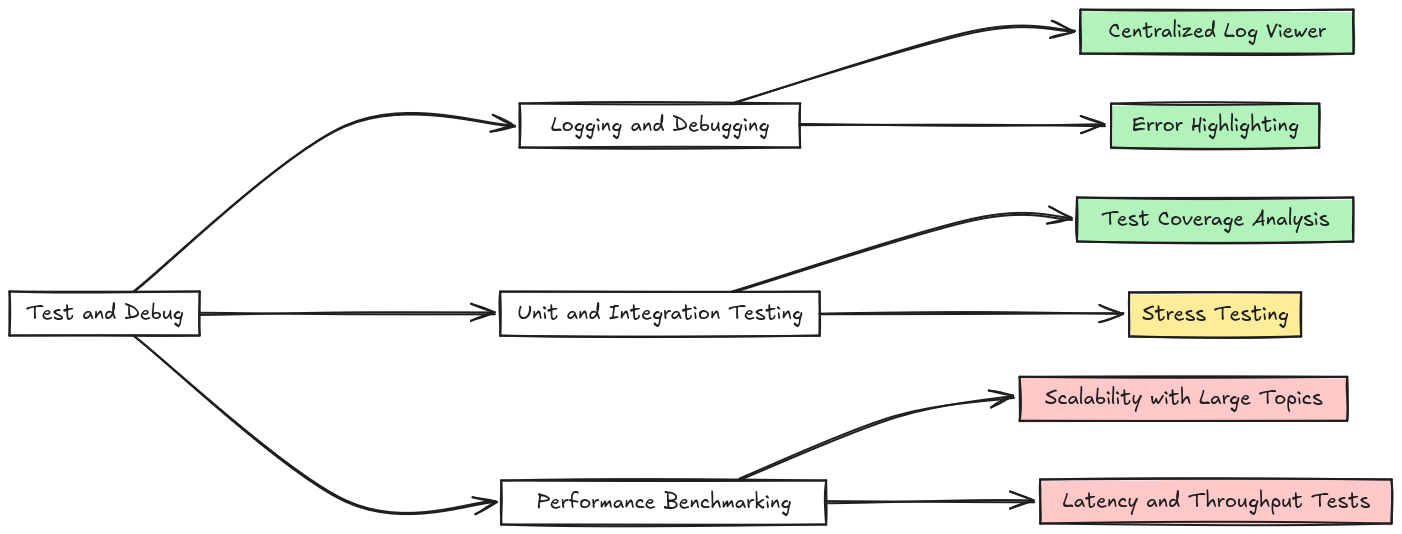
\includegraphics[width=1\linewidth]{imgs/TestDebugDiagram.png}
    \label{fig:enter-label}
\end{figure}


\begin{figure}
    \centering
    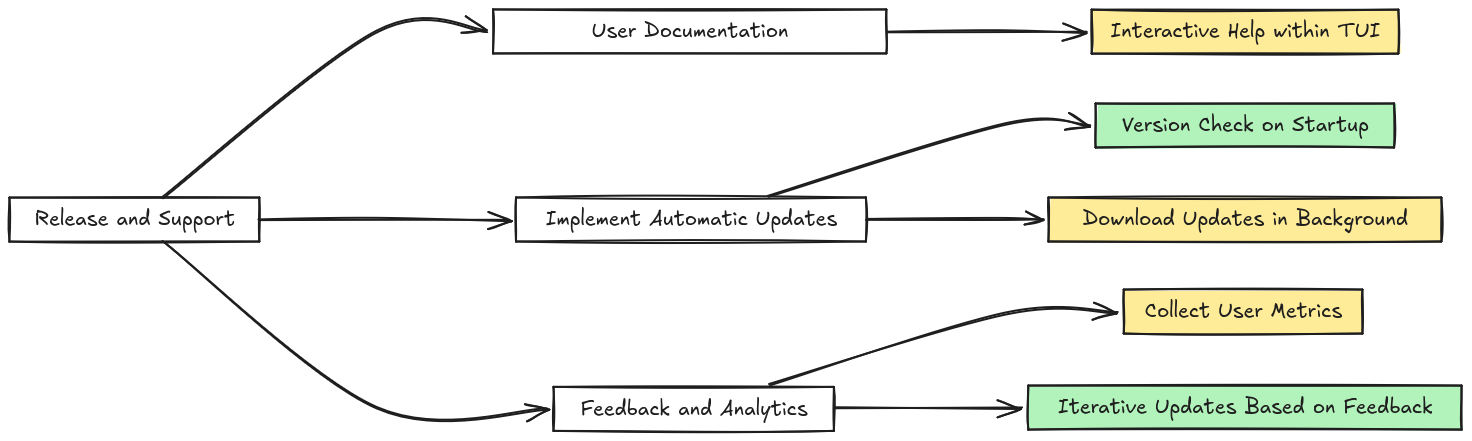
\includegraphics[width=1\linewidth]{imgs/ReleaseSupportDiagram.png}
    \label{fig:enter-label}
\end{figure}



\begin{figure}[htpb]
    \centering
    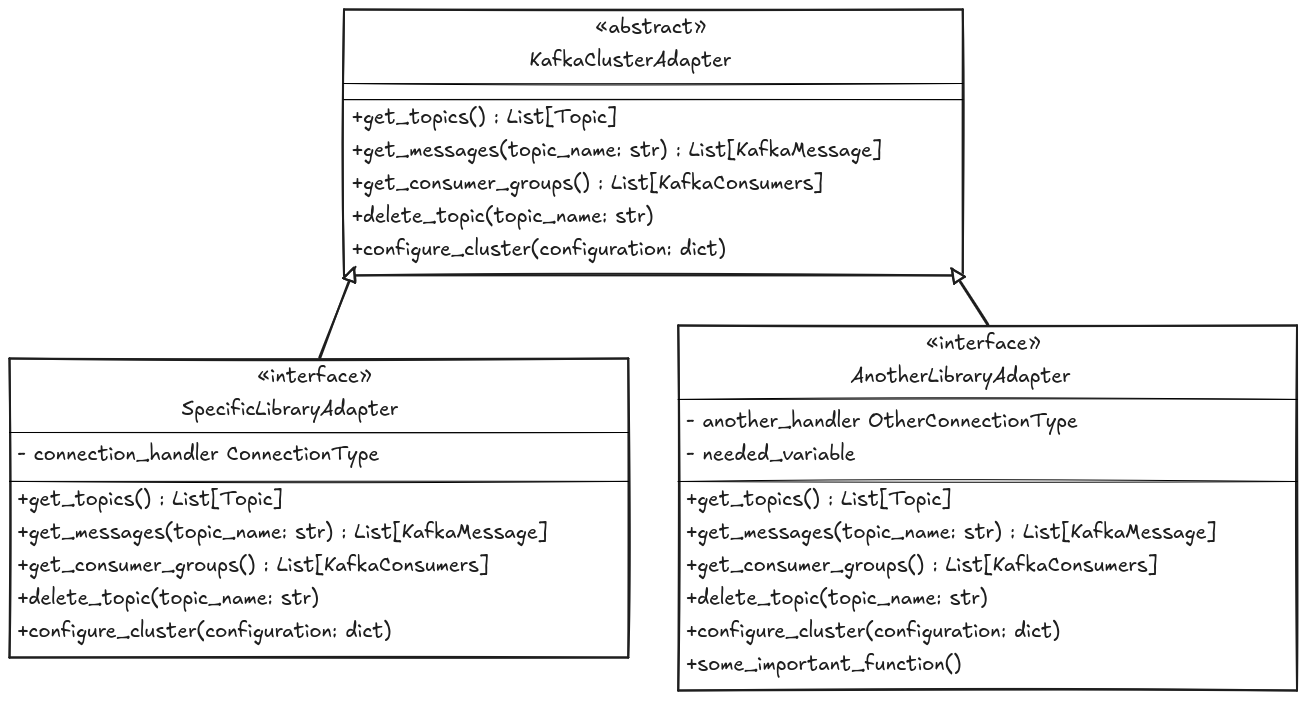
\includegraphics[width=1\linewidth]{imgs/AdapterUML.png}
    \caption{Adapter Example}
    \label{fig:AdapterUML}
\end{figure}

\appendix

\chapter{System Design}\label{appendix:system_design}
\begin{figure}[htpb]
    \centering
    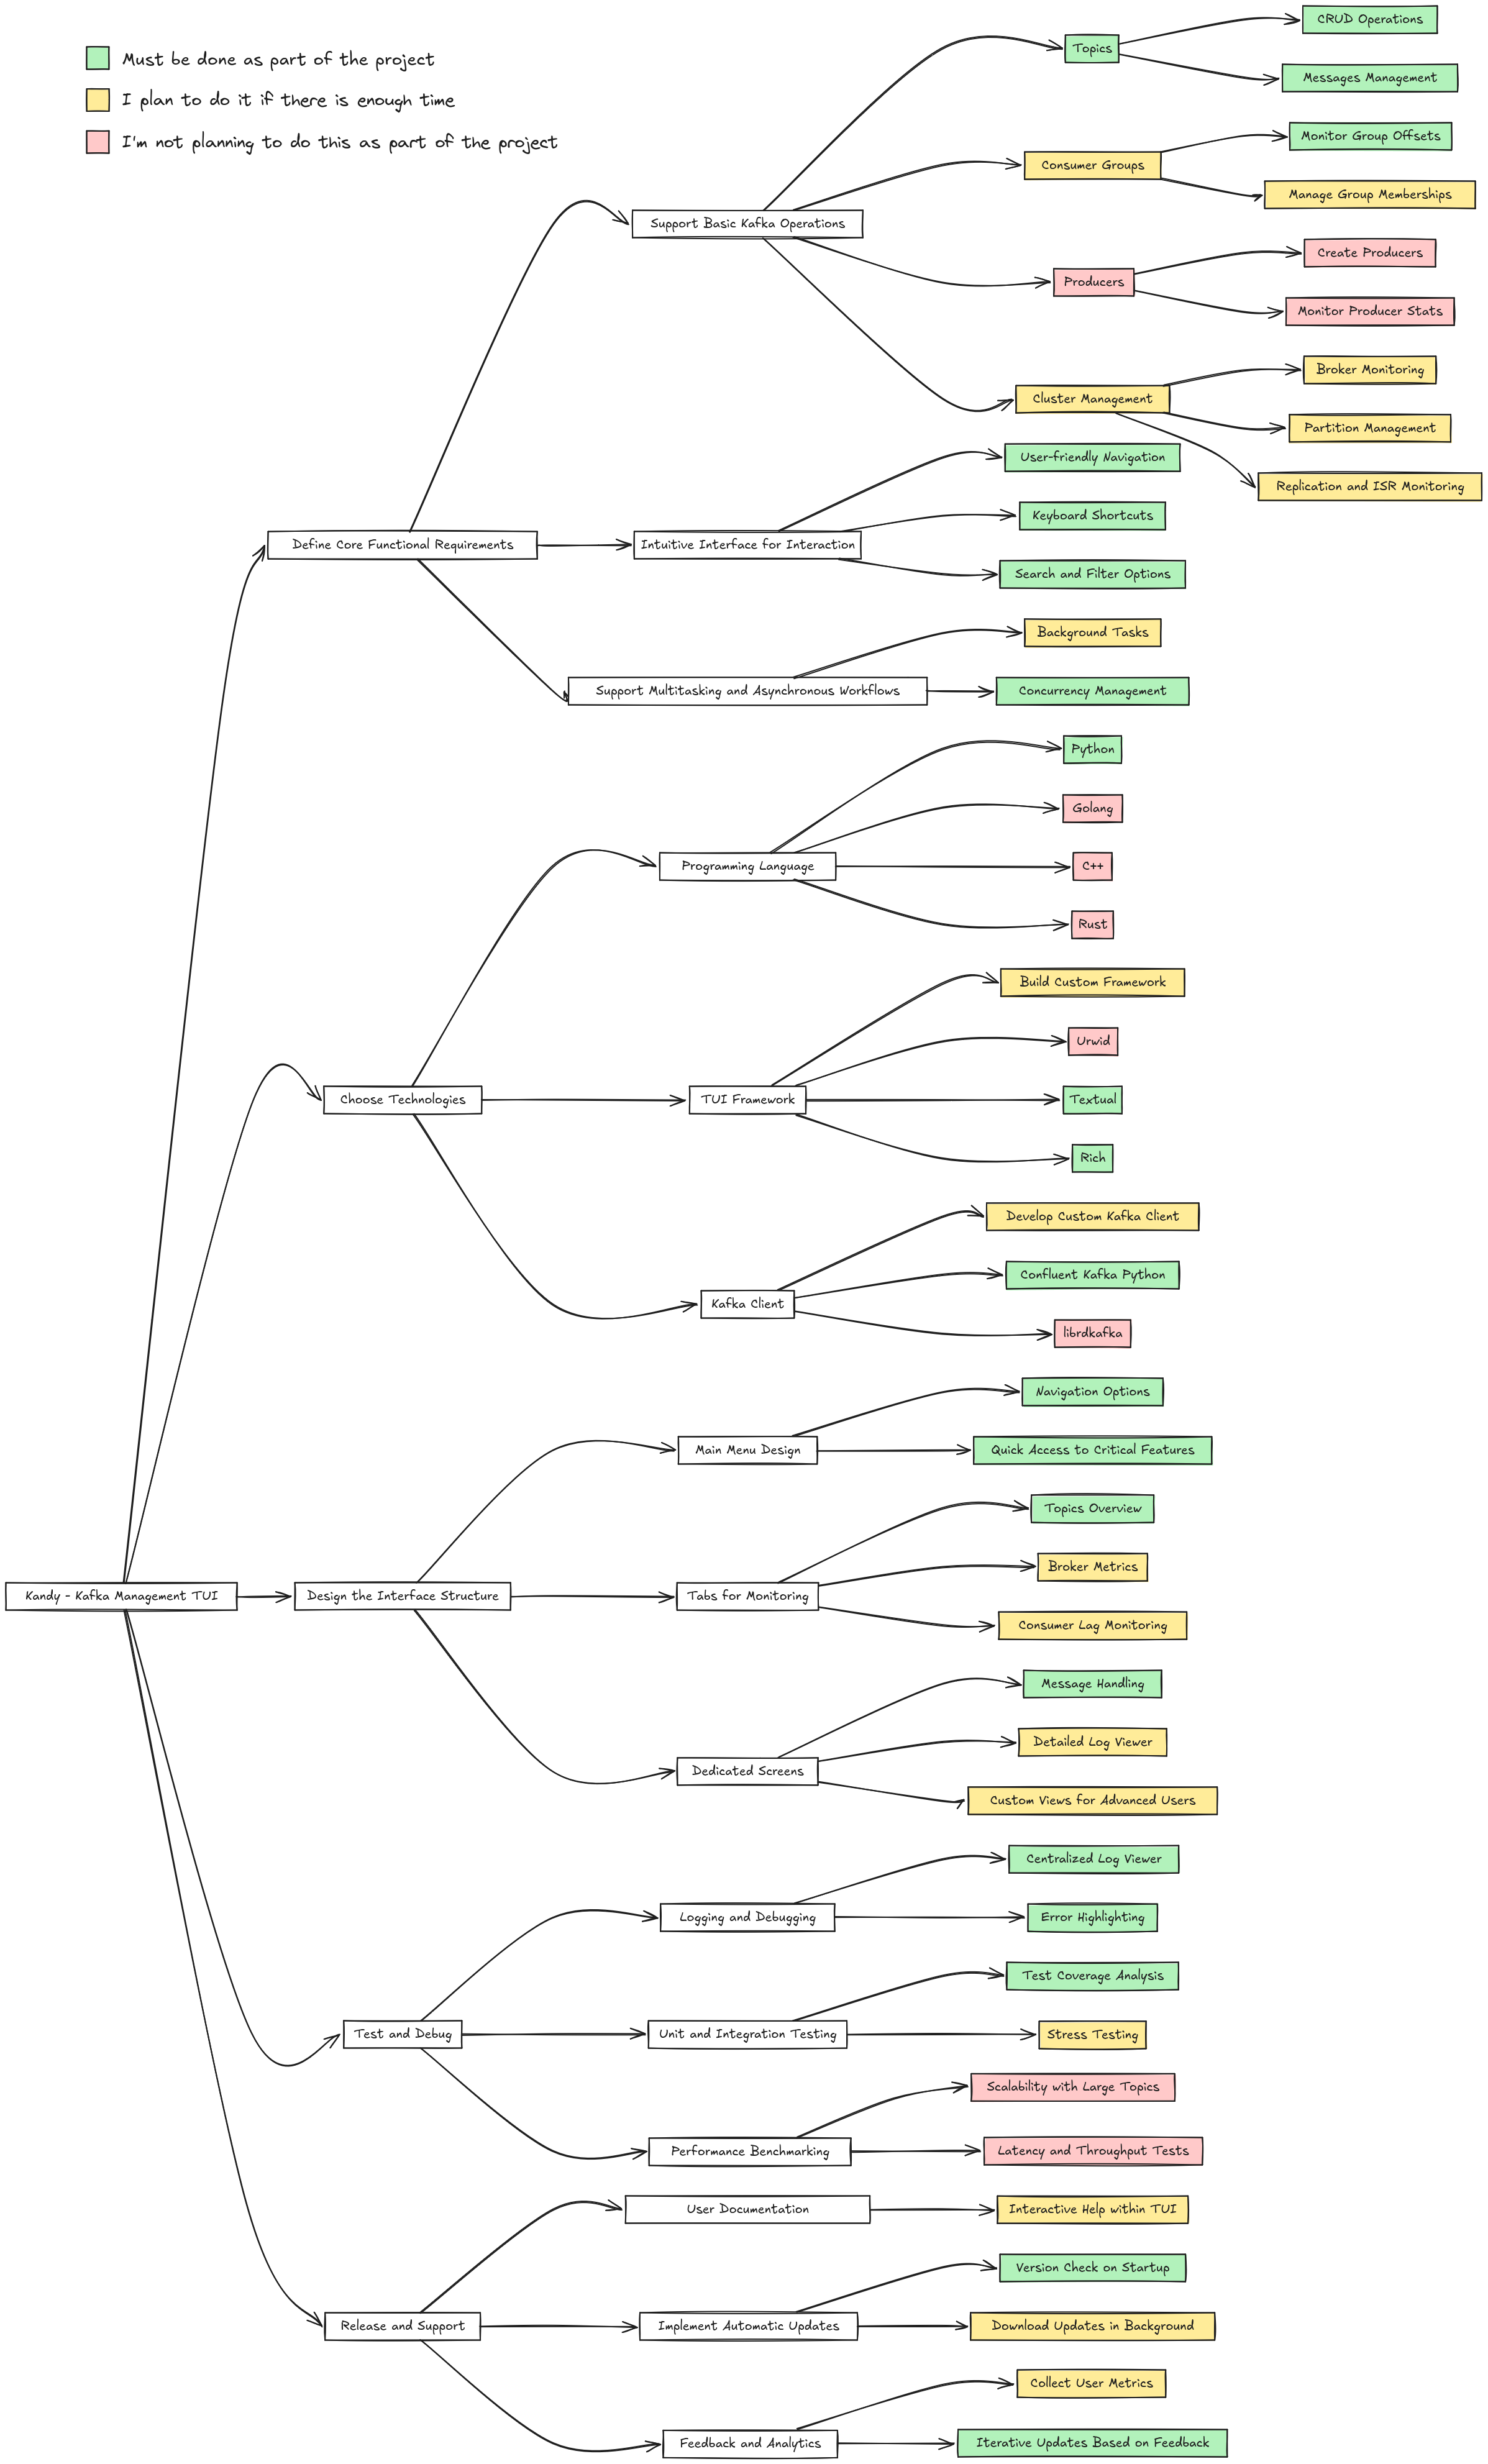
\includegraphics[width=0.9\linewidth]{imgs/SystemDesign.png}
\end{figure}

\chapter{Files}
\section{pyproject.toml (Libraries and dependencies)}\label{appendix:libs}
\begin{listing}[htbp]
    \begin{minted}{Python}
[tool.poetry]
name = "kandy-kafka"
version = "0.0.1"
description = "Handy way to manage kafka"
authors = ["Perchinka <alexsator.lukin@gmail.com>"]
license = "GPL-2.0-only"
readme = "README.md"

[tool.poetry.dependencies]
python = "^3.11"
confluent-kafka = "^2.3.0"
urwid = "^2.6.10"
panwid = "^0.3.5"
pydantic = "^2.6.4"
pyyaml = "^6.0.1"
textual = "^0.81.0"

[tool.poetry.dev-dependencies]
pytest = "^8.1.1"
pytest-bdd = "^7.1.2"
pytest-cov = "^5.0.0"

[build-system]
requires = ["poetry-core"]
build-backend = "poetry.core.masonry.api"
    \end{minted}
    \caption{pyproject.toml}
\end{listing}

\renewcommand{\bibname}{References}
\begin{thebibliography}{00}
\bibitem{b1} None yet
\end{thebibliography}

\end{document}
